\UseRawInputEncoding
%DIF LATEXDIFF DIFFERENCE FILE
%DIF DEL ./old/compiled_v003.tex   Sat Jan 13 16:40:13 2024
%DIF ADD ./compiled.tex            Sat Jan 13 16:44:47 2024

%%%%%%%%%%%%%%%%%%%%%%%%%%%%%%%%%%%%%%%%%%%%%%%%%%%%%%%%%%%%%%%%%%%%%%%%%%%%%%%%
%% SETTINGS
%%%%%%%%%%%%%%%%%%%%%%%%%%%%%%%%%%%%%%%%%%%%%%%%%%%%%%%%%%%%%%%%%%%%%%%%%%%%%%%%
%% Columns
\documentclass[final,3p,times,twocolumn]{elsarticle}
%% Use the options 1p,twocolumn; 3p; 3p,twocolumn; 5p; or 5p,twocolumn
%% for a journal layout:
%% \documentclass[final,1p,times]{elsarticle}
%% \documentclass[final,1p,times,twocolumn]{elsarticle}
%% \documentclass[final,3p,times]{elsarticle}
%% \documentclass[final,3p,times,twocolumn]{elsarticle}
%% \documentclass[final,5p,times]{elsarticle}
%% \documentclass[final,5p,times,twocolumn]{elsarticle}
%% \documentclass[preprint,review,12pt]{elsarticle}

%% Image width
\newlength{\imagewidth}
\newlength{\imagescale}
%% preamble
\usepackage[english]{babel}
\usepackage[table]{xcolor} % For coloring tables
\usepackage{booktabs} % For professional quality tables
\usepackage{colortbl} % For coloring cells in tables
\usepackage{amsmath, amssymb} % For mathematical symbols and environments
\usepackage{amsthm} % For theorem-like environments
\usepackage{lipsum} % just for sample text
\usepackage{natbib}
\usepackage{graphicx}
\usepackage{indentfirst}
\usepackage{bashful}
\usepackage[margin=10pt,font=small,labelfont=bf,labelsep=endash]{caption}
\usepackage{graphicx}
\usepackage{calc}
\usepackage[T1]{fontenc} % [REVISED]
\usepackage[utf8]{inputenc} % [REVISED]
\usepackage{hyperref}
\usepackage{accsupp}
%% Line numbers
\linespread{1.1}
% \linenumbers
% Tables
\usepackage[pass]{geometry}
\usepackage{pdflscape}
\usepackage{csvsimple}
\usepackage{xltabular}
\usepackage{booktabs}
\usepackage{siunitx}
\usepackage{makecell}
\sisetup{round-mode=figures,round-precision=3}
\renewcommand\theadfont{\bfseries}
\renewcommand\theadalign{c}
\newcolumntype{C}[1]{>{\centering\arraybackslash}m{#1}}
\renewcommand{\arraystretch}{1.5}
\definecolor{lightgray}{gray}{0.95}

%% Diff
\usepackage{xcolor}
% Define commands for highlighting
% diff
\usepackage[most]{tcolorbox} % for boxes with transparency
% Define colors with transparency (opacity value)
\definecolor{GreenBG}{rgb}{0,1,0}
\definecolor{RedBG}{rgb}{1,0,0}
% Define tcolorbox environments for highlighting
\newtcbox{\greenhighlight}[1][]{%
  on line,
  colframe=GreenBG,
  colback=GreenBG!50!white, % 50% transparent green
  boxrule=0pt,
  arc=0pt,
  boxsep=0pt,
  left=1pt,
  right=1pt,
  top=2pt,
  bottom=2pt,
  tcbox raise base
}
\newtcbox{\redhighlight}[1][]{%
  on line,
  colframe=RedBG,
  colback=RedBG!50!white, % 50% transparent red
  boxrule=0pt,
  arc=0pt,
  boxsep=0pt,
  left=1pt,
  right=1pt,
  top=2pt,
  bottom=2pt,
  tcbox raise base
}
\newcommand{\REDSTARTS}{\color{red}}
\newcommand{\REDENDS}{\color{black}}
\newcommand{\GREENSTARTS}{\color{green}}
\newcommand{\GREENENDS}{\color{black}}
%%%%%%%%%%%%%%%%%%%%%%%%%%%%%%%%%%%%%%%%%%%%%%%%%%%%%%%%%%%%%%%%%%%%%%%%%%%%%%%%
%% JOURNAL NAME
%%%%%%%%%%%%%%%%%%%%%%%%%%%%%%%%%%%%%%%%%%%%%%%%%%%%%%%%%%%%%%%%%%%%%%%%%%%%%%%%
\journal{Heliyon}
%%%%%%%%%%%%%%%%%%%%%%%%%%%%%%%%%%%%%%%%%%%%%%%%%%%%%%%%%%%%%%%%%%%%%%%%%%%%%%%%
%% DOCUMENT STARTS
%%%%%%%%%%%%%%%%%%%%%%%%%%%%%%%%%%%%%%%%%%%%%%%%%%%%%%%%%%%%%%%%%%%%%%%%%%%%%%%%
%DIF PREAMBLE EXTENSION ADDED BY LATEXDIFF
%DIF UNDERLINE PREAMBLE %DIF PREAMBLE
\RequirePackage[normalem]{ulem} %DIF PREAMBLE
\RequirePackage{color}\definecolor{RED}{rgb}{1,0,0}\definecolor{BLUE}{rgb}{0,0,1} %DIF PREAMBLE
\providecommand{\DIFaddtex}[1]{{\protect\color{blue}\uwave{#1}}} %DIF PREAMBLE
\providecommand{\DIFdeltex}[1]{{\protect\color{red}\sout{#1}}}                      %DIF PREAMBLE
%DIF SAFE PREAMBLE %DIF PREAMBLE
\providecommand{\DIFaddbegin}{} %DIF PREAMBLE
\providecommand{\DIFaddend}{} %DIF PREAMBLE
\providecommand{\DIFdelbegin}{} %DIF PREAMBLE
\providecommand{\DIFdelend}{} %DIF PREAMBLE
\providecommand{\DIFmodbegin}{} %DIF PREAMBLE
\providecommand{\DIFmodend}{} %DIF PREAMBLE
%DIF FLOATSAFE PREAMBLE %DIF PREAMBLE
\providecommand{\DIFaddFL}[1]{\DIFadd{#1}} %DIF PREAMBLE
\providecommand{\DIFdelFL}[1]{\DIFdel{#1}} %DIF PREAMBLE
\providecommand{\DIFaddbeginFL}{} %DIF PREAMBLE
\providecommand{\DIFaddendFL}{} %DIF PREAMBLE
\providecommand{\DIFdelbeginFL}{} %DIF PREAMBLE
\providecommand{\DIFdelendFL}{} %DIF PREAMBLE
%DIF HYPERREF PREAMBLE %DIF PREAMBLE
\providecommand{\DIFadd}[1]{\texorpdfstring{\DIFaddtex{#1}}{#1}} %DIF PREAMBLE
\providecommand{\DIFdel}[1]{\texorpdfstring{\DIFdeltex{#1}}{}} %DIF PREAMBLE
\newcommand{\DIFscaledelfig}{0.5}
%DIF HIGHLIGHTGRAPHICS PREAMBLE %DIF PREAMBLE
\RequirePackage{settobox} %DIF PREAMBLE
\RequirePackage{letltxmacro} %DIF PREAMBLE
\newsavebox{\DIFdelgraphicsbox} %DIF PREAMBLE
\newlength{\DIFdelgraphicswidth} %DIF PREAMBLE
\newlength{\DIFdelgraphicsheight} %DIF PREAMBLE
% store original definition of \includegraphics %DIF PREAMBLE
\LetLtxMacro{\DIFOincludegraphics}{\includegraphics} %DIF PREAMBLE
\newcommand{\DIFaddincludegraphics}[2][]{{\color{blue}\fbox{\DIFOincludegraphics[#1]{#2}}}} %DIF PREAMBLE
\newcommand{\DIFdelincludegraphics}[2][]{% %DIF PREAMBLE
\sbox{\DIFdelgraphicsbox}{\DIFOincludegraphics[#1]{#2}}% %DIF PREAMBLE
\settoboxwidth{\DIFdelgraphicswidth}{\DIFdelgraphicsbox} %DIF PREAMBLE
\settoboxtotalheight{\DIFdelgraphicsheight}{\DIFdelgraphicsbox} %DIF PREAMBLE
\scalebox{\DIFscaledelfig}{% %DIF PREAMBLE
\parbox[b]{\DIFdelgraphicswidth}{\usebox{\DIFdelgraphicsbox}\\[-\baselineskip] \rule{\DIFdelgraphicswidth}{0em}}\llap{\resizebox{\DIFdelgraphicswidth}{\DIFdelgraphicsheight}{% %DIF PREAMBLE
\setlength{\unitlength}{\DIFdelgraphicswidth}% %DIF PREAMBLE
\begin{picture}(1,1)% %DIF PREAMBLE
\thicklines\linethickness{2pt} %DIF PREAMBLE
{\color[rgb]{1,0,0}\put(0,0){\framebox(1,1){}}}% %DIF PREAMBLE
{\color[rgb]{1,0,0}\put(0,0){\line( 1,1){1}}}% %DIF PREAMBLE
{\color[rgb]{1,0,0}\put(0,1){\line(1,-1){1}}}% %DIF PREAMBLE
\end{picture}% %DIF PREAMBLE
}\hspace*{3pt}}} %DIF PREAMBLE
} %DIF PREAMBLE
\LetLtxMacro{\DIFOaddbegin}{\DIFaddbegin} %DIF PREAMBLE
\LetLtxMacro{\DIFOaddend}{\DIFaddend} %DIF PREAMBLE
\LetLtxMacro{\DIFOdelbegin}{\DIFdelbegin} %DIF PREAMBLE
\LetLtxMacro{\DIFOdelend}{\DIFdelend} %DIF PREAMBLE
\DeclareRobustCommand{\DIFaddbegin}{\DIFOaddbegin \let\includegraphics\DIFaddincludegraphics} %DIF PREAMBLE
\DeclareRobustCommand{\DIFaddend}{\DIFOaddend \let\includegraphics\DIFOincludegraphics} %DIF PREAMBLE
\DeclareRobustCommand{\DIFdelbegin}{\DIFOdelbegin \let\includegraphics\DIFdelincludegraphics} %DIF PREAMBLE
\DeclareRobustCommand{\DIFdelend}{\DIFOaddend \let\includegraphics\DIFOincludegraphics} %DIF PREAMBLE
\LetLtxMacro{\DIFOaddbeginFL}{\DIFaddbeginFL} %DIF PREAMBLE
\LetLtxMacro{\DIFOaddendFL}{\DIFaddendFL} %DIF PREAMBLE
\LetLtxMacro{\DIFOdelbeginFL}{\DIFdelbeginFL} %DIF PREAMBLE
\LetLtxMacro{\DIFOdelendFL}{\DIFdelendFL} %DIF PREAMBLE
\DeclareRobustCommand{\DIFaddbeginFL}{\DIFOaddbeginFL \let\includegraphics\DIFaddincludegraphics} %DIF PREAMBLE
\DeclareRobustCommand{\DIFaddendFL}{\DIFOaddendFL \let\includegraphics\DIFOincludegraphics} %DIF PREAMBLE
\DeclareRobustCommand{\DIFdelbeginFL}{\DIFOdelbeginFL \let\includegraphics\DIFdelincludegraphics} %DIF PREAMBLE
\DeclareRobustCommand{\DIFdelendFL}{\DIFOaddendFL \let\includegraphics\DIFOincludegraphics} %DIF PREAMBLE
%DIF LISTINGS PREAMBLE %DIF PREAMBLE
\RequirePackage{listings} %DIF PREAMBLE
\RequirePackage{color} %DIF PREAMBLE
\lstdefinelanguage{DIFcode}{ %DIF PREAMBLE
%DIF DIFCODE_UNDERLINE %DIF PREAMBLE
  moredelim=[il][\color{red}\sout]{\%DIF\ <\ }, %DIF PREAMBLE
  moredelim=[il][\color{blue}\uwave]{\%DIF\ >\ } %DIF PREAMBLE
} %DIF PREAMBLE
\lstdefinestyle{DIFverbatimstyle}{ %DIF PREAMBLE
	language=DIFcode, %DIF PREAMBLE
	basicstyle=\ttfamily, %DIF PREAMBLE
	columns=fullflexible, %DIF PREAMBLE
	keepspaces=true %DIF PREAMBLE
} %DIF PREAMBLE
\lstnewenvironment{DIFverbatim}{\lstset{style=DIFverbatimstyle}}{} %DIF PREAMBLE
\lstnewenvironment{DIFverbatim*}{\lstset{style=DIFverbatimstyle,showspaces=true}}{} %DIF PREAMBLE
%DIF END PREAMBLE EXTENSION ADDED BY LATEXDIFF

\begin{document}

%%%%%%%%%%%%%%%%%%%%%%%%%%%%%%%%%%%%%%%%%%%%%%%%%%%%%%%%%%%%%%%%%%%%%%%%%%%%%%%%
%% Frontmatter
%%%%%%%%%%%%%%%%%%%%%%%%%%%%%%%%%%%%%%%%%%%%%%%%%%%%%%%%%%%%%%%%%%%%%%%%%%%%%%%%
\begin{frontmatter}
\begin{highlights}
\pdfbookmark[1]{Highlights}{highlights}

\item Neural trajectories in the hippocampus exhibited greater variability during a working memory (WM) task compared to those in the entorhinal cortex and amygdala regions.

\item The distance of neural trajectories between encoding and retrieval states in the hippocampus was memory-load dependent during a WM task.


\item Hippocampal neural trajectories fluctuated between the encoding and retrieval states in a task-dependent manner during both baseline and sharp-wave ripple (SWR) periods.

\item Hippocampal neural trajectories shifted from encoding to retrieval states during SWR period.

\end{highlights}\title{
Hippocampal neural fluctuations between memory encoding and retrieval states during a working memory task in humans
}\author[1]{Yusuke Watanabe\corref{cor1}}
\author[2,3,4]{Yuji Ikegaya}
\author[1,5]{Takufumi Yanagisawa}

\address[1]{Institute for Advanced Cocreation studies, Osaka University, 2-2 Yamadaoka, Suita, 565-0871, Osaka, Japan}
\address[2]{Graduate School of Pharmaceutical Sciences, The University of Tokyo, 7-3-1 Hongo, Tokyo, 113-0033, Japan}
\address[3]{Institute for AI and Beyond, The University of Tokyo, 7-3-1 Hongo, Tokyo, 113-0033, Japan}
\address[4]{Center for Information and Neural Networks, National Institute of Information and Communications Technology, 1-4 Yamadaoka, Suita City, 565-0871, Osaka, Japan}
\address[5]{Department of Neurosurgery, Osaka University Graduate School of Medicine, 2-2 Yamadaoka, Osaka, 565-0871, Japan}

\cortext[cor1]{Corresponding author. Tel: +81-6-6879-3652}%%Graphical abstract
%\pdfbookmark[1]{Graphical Abstract}{graphicalabstract}        
%\begin{graphicalabstract}
%\includegraphics{grabs}
%\end{graphicalabstract}
\begin{abstract}
\pdfbookmark[1]{Abstract}{abstract}
\DIFdelbegin \DIFdel{The working }\DIFdelend \DIFaddbegin \DIFadd{Working }\DIFaddend memory (WM), \DIFdelbegin \DIFdel{a cornerstone of many }\DIFdelend \DIFaddbegin \DIFadd{critical to various }\DIFaddend cognitive functions, \DIFdelbegin \DIFdel{holds complex neural mechanisms that are not yet }\DIFdelend \DIFaddbegin \DIFadd{embodies intricate neural mechanisms which are not }\DIFaddend entirely understood. \DIFdelbegin \DIFdel{Specifically, the involvement }\DIFdelend \DIFaddbegin \DIFadd{Notably, the role }\DIFaddend of the hippocampus and sharp-wave ripple complexes (SWRs) -- \DIFdelbegin \DIFdel{rapid, coincident neural }\DIFdelend \DIFaddbegin \DIFadd{coordinated, rapid neuronal }\DIFaddend events within the hippocampus -- in WM tasks remains somewhat \DIFdelbegin \DIFdel{uncertain, despite their established roles }\DIFdelend \DIFaddbegin \DIFadd{ambiguous, notwithstanding their confirmed involvement }\DIFaddend in memory consolidation and retrieval. In our \DIFdelbegin \DIFdel{current }\DIFdelend \DIFaddbegin \DIFadd{present }\DIFaddend research, we \DIFdelbegin \DIFdel{propose }\DIFdelend \DIFaddbegin \DIFadd{posit }\DIFaddend that multiunit activity patterns within the hippocampus \DIFdelbegin \DIFdel{interact }\DIFdelend \DIFaddbegin \DIFadd{operate }\DIFaddend synergistically with SWRs, \DIFdelbegin \DIFdel{thereby displaying unique }\DIFdelend \DIFaddbegin \DIFadd{consequently exhibiting distinctive }\DIFaddend dynamics during WM tasks. \DIFdelbegin \DIFdel{This study involved an extensive }\DIFdelend \DIFaddbegin \DIFadd{Our study engaged in a comprehensive }\DIFaddend analysis of a dataset \DIFdelbegin \DIFdel{obtained }\DIFdelend \DIFaddbegin \DIFadd{derived }\DIFaddend from intracranial electroencephalogram recordings from the medial temporal \DIFdelbegin \DIFdel{lobe }\DIFdelend \DIFaddbegin \DIFadd{lobes }\DIFaddend (MTL) of nine \DIFdelbegin \DIFdel{patients with epilepsy, while performing }\DIFdelend \DIFaddbegin \DIFadd{epileptic patients executing }\DIFaddend an eight-second Sternberg task. Gaussian-process factor analysis was \DIFdelbegin \DIFdel{employed to identify }\DIFdelend \DIFaddbegin \DIFadd{utilized to pinpoint }\DIFaddend low-dimensional neural \DIFdelbegin \DIFdel{representations}\DIFdelend \DIFaddbegin \DIFadd{vectors}\DIFaddend , or 'trajectories,' within the MTL during the WM task. We \DIFdelbegin \DIFdel{found }\DIFdelend \DIFaddbegin \DIFadd{discovered }\DIFaddend that the hippocampus \DIFdelbegin \DIFdel{exhibited the most significant variations }\DIFdelend \DIFaddbegin \DIFadd{showed the most pronounced variation }\DIFaddend in neural trajectories \DIFdelbegin \DIFdel{compared }\DIFdelend \DIFaddbegin \DIFadd{relative }\DIFaddend to the entorhinal cortex and the amygdala. \DIFdelbegin \DIFdel{Interestingly, the divergence }\DIFdelend \DIFaddbegin \DIFadd{Intriguingly, the deviation }\DIFaddend in trajectories between \DIFaddbegin \DIFadd{the }\DIFaddend encoding and retrieval phases was \DIFdelbegin \DIFdel{memory load-dependent. More specifically}\DIFdelend \DIFaddbegin \DIFadd{seen to be dependent on memory load. Further}\DIFaddend , hippocampal trajectories \DIFdelbegin \DIFdel{oscillated }\DIFdelend \DIFaddbegin \DIFadd{showed oscillatory behavior }\DIFaddend during the retrieval phase, \DIFdelbegin \DIFdel{revealing task-dependent }\DIFdelend \DIFaddbegin \DIFadd{indicating task-related }\DIFaddend transitions between encoding and retrieval states, \DIFdelbegin \DIFdel{encapsulating }\DIFdelend \DIFaddbegin \DIFadd{and embracing both }\DIFaddend baseline and SWR episodes. These oscillations \DIFdelbegin \DIFdel{moved }\DIFdelend \DIFaddbegin \DIFadd{transitioned }\DIFaddend from encoding to retrieval states \DIFdelbegin \DIFdel{correlating }\DIFdelend \DIFaddbegin \DIFadd{in correlation }\DIFaddend with the SWRs. \DIFdelbegin \DIFdel{Therefore}\DIFdelend \DIFaddbegin \DIFadd{Hence}\DIFaddend , these findings \DIFdelbegin \DIFdel{emphasize the essential }\DIFdelend \DIFaddbegin \DIFadd{underscore the crucial }\DIFaddend role of the hippocampus in \DIFdelbegin \DIFdel{performing }\DIFdelend \DIFaddbegin \DIFadd{tackling }\DIFaddend WM tasks and \DIFdelbegin \DIFdel{suggest a compelling premise for further investigation}\DIFdelend \DIFaddbegin \DIFadd{propose an enticing hypothesis for future exploration}\DIFaddend : the functional state of the hippocampus \DIFdelbegin \DIFdel{transitions }\DIFdelend \DIFaddbegin \DIFadd{switches }\DIFaddend from encoding to retrieval during SWRs.
\end{abstract}% \pdfbookmark[1]{Keywords}{keywords}                
\begin{keyword}
working memory \sep WM \sep memory load \sep hippocampus \sep sharp-wave ripples \sep SWR \sep humans
\end{keyword}
\end{frontmatter}

%%%%%%%%%%%%%%%%%%%%%%%%%%%%%%%%%%%%%%%%%%%%%%%%%%%%%%%%%%%%%%%%%%%%%%%%%%%%%%%%
%% IMRaD
%%%%%%%%%%%%%%%%%%%%%%%%%%%%%%%%%%%%%%%%%%%%%%%%%%%%%%%%%%%%%%%%%%%%%%%%%%%%%%%%

%%%%%%%%%%%%%%%%%%%%%%%%%%%%%%%%%%%%%%%%%%%%%%%%%%%%%%%%%%%%%%%%%%%%%%%%%%%%%%%%
%% INTRODUCTION
%%%%%%%%%%%%%%%%%%%%%%%%%%%%%%%%%%%%%%%%%%%%%%%%%%%%%%%%%%%%%%%%%%%%%%%%%%%%%%%%
Working memory (WM) \DIFdelbegin \DIFdel{plays a crucial }\DIFdelend \DIFaddbegin \DIFadd{serves a critical }\DIFaddend role in everyday life, \DIFdelbegin \DIFdel{and its neural underpinnings remain an area of ongoing research}\DIFdelend \DIFaddbegin \DIFadd{with its neural foundations being an ongoing subject of study}\DIFaddend . The hippocampus, \DIFdelbegin \DIFdel{notably integral to memory , continues to be a primary focus of this investigation }\DIFdelend \DIFaddbegin \DIFadd{particularly crucial to memory function, remains central to this research }\DIFaddend \cite{scoville_loss_1957} \cite{squire_legacy_2009}  \cite{boran_persistent_2019} \cite{kaminski_persistently_2017} \cite{kornblith_persistent_2017} \cite{faraut_dataset_2018} \cite{borders_hippocampus_2022} \cite{li_functional_2023} \cite{dimakopoulos_information_2022}. \DIFdelbegin \DIFdel{Gaining insights into }\DIFdelend \DIFaddbegin \DIFadd{Understanding }\DIFaddend the role of the hippocampus in working memory is \DIFdelbegin \DIFdel{vital to deepening our understanding }\DIFdelend \DIFaddbegin \DIFadd{essential to advancing our comprehension }\DIFaddend of cognitive processes, \DIFdelbegin \DIFdel{hence fostering the progression of }\DIFdelend \DIFaddbegin \DIFadd{thereby promoting }\DIFaddend cognitive training and interventions.
\\
\indent
Current evidence \DIFdelbegin \DIFdel{suggests a transient}\DIFdelend \DIFaddbegin \DIFadd{points toward a brief}\DIFaddend , synchronized oscillation, \DIFdelbegin \DIFdel{referred to }\DIFdelend \DIFaddbegin \DIFadd{known }\DIFaddend as sharp-wave ripple (SWR) \cite{buzsaki_hippocampal_2015}, \DIFdelbegin \DIFdel{is linked }\DIFdelend \DIFaddbegin \DIFadd{being associated }\DIFaddend with several cognitive functions\DIFdelbegin \DIFdel{, such as }\DIFdelend \DIFaddbegin \DIFadd{. These include }\DIFaddend memory replay \cite{wilson_reactivation_1994} \cite{nadasdy_replay_1999} \cite{lee_memory_2002} \cite{diba_forward_2007} \cite{davidson_hippocampal_2009}, memory consolidation \cite{girardeau_selective_2009} \cite{ego-stengel_disruption_2010} \cite{fernandez-ruiz_long-duration_2019} \cite{kim_corticalhippocampal_2022}, memory recall \cite{wu_hippocampal_2017} \cite{norman_hippocampal_2019} \cite{norman_hippocampal_2021}, and neural plasticity \cite{behrens_induction_2005} \cite{norimoto_hippocampal_2018}. This \DIFdelbegin \DIFdel{evidence indicates the likelihood that SWR could be a critical component of }\DIFdelend \DIFaddbegin \DIFadd{suggests that SWR may play a crucial part in }\DIFaddend hippocampal processing, contributing to \DIFdelbegin \DIFdel{working memory performance}\DIFdelend \DIFaddbegin \DIFadd{the performance of working memory}\DIFaddend . However, \DIFdelbegin \DIFdel{research }\DIFdelend \DIFaddbegin \DIFadd{studies }\DIFaddend investigating the effects of SWRs on working memory \DIFdelbegin \DIFdel{remains sparse \mbox{%DIFAUXCMD
\cite{jadhav_awake_2012} }\hspace{0pt}%DIFAUXCMD
, and is largely limited to rodent models participating }\DIFdelend \DIFaddbegin \DIFadd{are limited \mbox{%DIFAUXCMD
\cite{jadhav_awake_2012} }\hspace{0pt}%DIFAUXCMD
and focus primarily on rodent models engaged }\DIFaddend in navigation tasks\DIFdelbegin \DIFdel{where the timing }\DIFdelend \DIFaddbegin \DIFadd{, without clear delineation }\DIFaddend of memory acquisition and recall \DIFdelbegin \DIFdel{is not explicitly distinguished}\DIFdelend \DIFaddbegin \DIFadd{timing}\DIFaddend .
\\
\indent
Recent studies \DIFdelbegin \DIFdel{indicate }\DIFdelend \DIFaddbegin \DIFadd{have illustrated }\DIFaddend that hippocampal neurons \DIFdelbegin \DIFdel{exhibit }\DIFdelend \DIFaddbegin \DIFadd{present }\DIFaddend low-dimensional representations during WM tasks. \DIFdelbegin \DIFdel{Notably}\DIFdelend \DIFaddbegin \DIFadd{Specifically}\DIFaddend , the firing patterns of place cells \cite{okeefe_hippocampus_1971} \cite{okeefe_place_1976} \cite{ekstrom_cellular_2003} \cite{kjelstrup_finite_2008} \cite{harvey_intracellular_2009}, located in the hippocampus, \DIFdelbegin \DIFdel{are observed to be encompassed }\DIFdelend \DIFaddbegin \DIFadd{appear }\DIFaddend within a dynamic, nonlinear three-dimensional hyperbolic geometry in \DIFdelbegin \DIFdel{rodents \mbox{%DIFAUXCMD
\cite{zhang_hippocampal_2022}}\hspace{0pt}%DIFAUXCMD
. Moreover}\DIFdelend \DIFaddbegin \DIFadd{rodent models \mbox{%DIFAUXCMD
\cite{zhang_hippocampal_2022}}\hspace{0pt}%DIFAUXCMD
. Additionally}\DIFaddend , grid cells in the entorhinal cortex (EC)—the \DIFdelbegin \DIFdel{dominant pathway }\DIFdelend \DIFaddbegin \DIFadd{main route }\DIFaddend to the hippocampus \cite{naber_reciprocal_2001} \cite{van_strien_anatomy_2009} \cite{strange_functional_2014}—\DIFdelbegin \DIFdel{displayed }\DIFdelend \DIFaddbegin \DIFadd{display a }\DIFaddend toroidal topology during exploration \cite{gardner_toroidal_2022}. \DIFdelbegin \DIFdel{Unfortunately, these investigations are confined }\DIFdelend \DIFaddbegin \DIFadd{Regrettably, these studies are limited }\DIFaddend to spatial navigation tasks in rodents, \DIFdelbegin \DIFdel{thus imposing limitations on }\DIFdelend \DIFaddbegin \DIFadd{affecting }\DIFaddend the temporal resolution of WM tasks. The \DIFdelbegin \DIFdel{applicability }\DIFdelend \DIFaddbegin \DIFadd{application }\DIFaddend of these findings to human subjects and their \DIFdelbegin \DIFdel{generalization }\DIFdelend \DIFaddbegin \DIFadd{extension }\DIFaddend beyond navigation tasks \DIFdelbegin \DIFdel{remains to be established}\DIFdelend \DIFaddbegin \DIFadd{are still unconfirmed}\DIFaddend .
\\
\indent
\DIFdelbegin \DIFdel{Given these considerations, the current study aims to validate }\DIFdelend \DIFaddbegin \DIFadd{In light of these points, the present study seeks to corroborate }\DIFaddend the hypothesis that hippocampal neurons \DIFdelbegin \DIFdel{exhibit distinctive }\DIFdelend \DIFaddbegin \DIFadd{portray unique }\DIFaddend representations in low-dimensional spaces, \DIFdelbegin \DIFdel{designated }\DIFdelend \DIFaddbegin \DIFadd{referred to }\DIFaddend as 'neural trajectory,' \DIFdelbegin \DIFdel{during WM tasks, most prominently within SWR periods . To evaluate this claim, we employed a dataset of }\DIFdelend \DIFaddbegin \DIFadd{particularly during SWR periods in WM tasks. To test this proposition, we used a dataset from }\DIFaddend patients performing an eight-second Sternberg task \DIFdelbegin \DIFdel{with high temporal resolution }\DIFdelend (1 \DIFdelbegin \DIFdel{s }\DIFdelend \DIFaddbegin \DIFadd{second }\DIFaddend for fixation, 2 \DIFdelbegin \DIFdel{s }\DIFdelend \DIFaddbegin \DIFadd{seconds }\DIFaddend for encoding, 3 \DIFdelbegin \DIFdel{s }\DIFdelend \DIFaddbegin \DIFadd{seconds }\DIFaddend for maintenance, and 2 \DIFdelbegin \DIFdel{s }\DIFdelend \DIFaddbegin \DIFadd{seconds }\DIFaddend for retrieval) \DIFaddbegin \DIFadd{with a high temporal resolution}\DIFaddend , while their intracranial electroencephalography \DIFdelbegin \DIFdel{signals }\DIFdelend (iEEG) \DIFdelbegin \DIFdel{within }\DIFdelend \DIFaddbegin \DIFadd{signals in }\DIFaddend the medial temporal lobe (MTL) were \DIFdelbegin \DIFdel{being }\DIFdelend monitored \cite{boran_dataset_2020}. To \DIFdelbegin \DIFdel{investigate }\DIFdelend \DIFaddbegin \DIFadd{explore the }\DIFaddend low-dimensional neural trajectories, we \DIFdelbegin \DIFdel{employed }\DIFdelend \DIFaddbegin \DIFadd{utilized the }\DIFaddend Gaussian-process factor analysis (GPFA), a \DIFdelbegin \DIFdel{method renowned for analyzing }\DIFdelend \DIFaddbegin \DIFadd{recognized technique for examining }\DIFaddend neural population dynamics \cite{yu_gaussian-process_2009}.
\label{sec:introduction}
%%%%%%%%%%%%%%%%%%%%%%%%%%%%%%%%%%%%%%%%%%%%%%%%%%%%%%%%%%%%%%%%%%%%%%%%%%%%%%%%
%% METHODS
%%%%%%%%%%%%%%%%%%%%%%%%%%%%%%%%%%%%%%%%%%%%%%%%%%%%%%%%%%%%%%%%%%%%%%%%%%%%%%%%
\section{Methods}
\subsection{Dataset}
A \DIFdelbegin \DIFdel{publicly available dataset \mbox{%DIFAUXCMD
\cite{boran_dataset_2020} }\hspace{0pt}%DIFAUXCMD
was used, which consists of }\DIFdelend \DIFaddbegin \DIFadd{public dataset \mbox{%DIFAUXCMD
\cite{boran_dataset_2020} }\hspace{0pt}%DIFAUXCMD
comprising experiments from }\DIFaddend nine epilepsy patients \DIFdelbegin \DIFdel{performing }\DIFdelend \DIFaddbegin \DIFadd{was taken into consideration for this study. The patients were tasked with executing }\DIFaddend a modified Sternberg task \DIFdelbegin \DIFdel{. This task involves }\DIFdelend \DIFaddbegin \DIFadd{which included }\DIFaddend four phases: fixation (1s), encoding (2s), maintenance (3s), and retrieval (2s) \cite{boran_dataset_2020}. During the encoding phase, participants were \DIFdelbegin \DIFdel{exposed to }\DIFdelend \DIFaddbegin \DIFadd{presented with }\DIFaddend four, six, or eight alphabet letters, \DIFdelbegin \DIFdel{referred to }\DIFdelend \DIFaddbegin \DIFadd{known }\DIFaddend as the set size. Subsequently, they had to \DIFdelbegin \DIFdel{decide }\DIFdelend \DIFaddbegin \DIFadd{ascertain }\DIFaddend whether a probe letter \DIFdelbegin \DIFdel{presented }\DIFdelend \DIFaddbegin \DIFadd{revealed }\DIFaddend during the retrieval phase was \DIFdelbegin \DIFdel{previously displayed (the correct }\DIFdelend \DIFaddbegin \DIFadd{displayed earlier (the suitable }\DIFaddend choice for the Match IN task) or not (the \DIFdelbegin \DIFdel{correct }\DIFdelend \DIFaddbegin \DIFadd{suitable }\DIFaddend choice for the Mismatch OUT task). iEEG signals were \DIFdelbegin \DIFdel{recorded at }\DIFdelend \DIFaddbegin \DIFadd{registered via }\DIFaddend a sampling rate of 32 kHz, within a frequency \DIFdelbegin \DIFdel{range }\DIFdelend \DIFaddbegin \DIFadd{spectrum }\DIFaddend of 0.5--5,000 Hz, \DIFdelbegin \DIFdel{using }\DIFdelend \DIFaddbegin \DIFadd{utilizing }\DIFaddend depth electrodes implanted in the medial temporal lobe (MTL) regions: the anterior head of the left and \DIFdelbegin \DIFdel{the }\DIFdelend right hippocampus (AHL and AHR), the posterior body of the hippocampus (PHL and PHR), the entorhinal cortex (ECL and ECR), and the amygdala (AL and AR) \DIFdelbegin \DIFdel{, as illustrated in }\DIFdelend \DIFaddbegin \DIFadd{(}\DIFaddend Figure~\ref{fig:01}A and Table~\ref{tab:01}\DIFdelbegin \DIFdel{. The }\DIFdelend \DIFaddbegin \DIFadd{). The recorded }\DIFaddend iEEG signals were subsequently downsampled to a rate of 2 kHz. \DIFdelbegin \DIFdel{Correlations }\DIFdelend \DIFaddbegin \DIFadd{The interrelationship }\DIFaddend among variables such as set size and correct rate were \DIFdelbegin \DIFdel{investigated }\DIFdelend \DIFaddbegin \DIFadd{explored }\DIFaddend (Figure~\ref{fig:s01}S1). The timings of multiunit spikes were \DIFdelbegin \DIFdel{determined by }\DIFdelend \DIFaddbegin \DIFadd{identified using }\DIFaddend a spike sorting algorithm \cite{niediek_reliable_2016} \DIFdelbegin \DIFdel{using }\DIFdelend \DIFaddbegin \DIFadd{with }\DIFaddend the Combinato package (\url{https://github.com/jniediek/combinato}) (Figure~\ref{fig:01}C).

\subsection{Calculation of neural trajectories using GPFA}
Neural trajectories, \DIFdelbegin \DIFdel{also termed }\DIFdelend \DIFaddbegin \DIFadd{colloquially called }\DIFaddend 'factors' (Figure~\ref{fig:01}D), in the hippocampus, EC, and amygdala (Figure~\ref{fig:01}D) \DIFdelbegin \DIFdel{, were computed using GPFA \mbox{%DIFAUXCMD
\cite{yu_gaussian-process_2009}}\hspace{0pt}%DIFAUXCMD
}\DIFdelend \DIFaddbegin \DIFadd{were calculated utilizing GPFA \mbox{%DIFAUXCMD
\cite{yu_gaussian-process_2009}}\hspace{0pt}%DIFAUXCMD
, which was }\DIFaddend applied to the multiunit activity data \DIFdelbegin \DIFdel{for }\DIFdelend \DIFaddbegin \DIFadd{radiating from }\DIFaddend each session. \DIFdelbegin \DIFdel{GPFA was }\DIFdelend \DIFaddbegin \DIFadd{The computations were }\DIFaddend performed with the elephant package (\url{https://elephant.readthedocs.io/en/latest/reference/gpfa.html}). The bin size was set \DIFdelbegin \DIFdel{to }\DIFdelend \DIFaddbegin \DIFadd{at }\DIFaddend 50 ms, with no overlaps. Each factor was z-normalized across all sessions. The Euclidean distance from the origin ($O$) was \DIFdelbegin \DIFdel{then }\DIFdelend \DIFaddbegin \DIFadd{subsequently }\DIFaddend calculated (Figure~\ref{fig:01}E).
\\
\indent
For each trajectory \DIFdelbegin \DIFdel{within }\DIFdelend \DIFaddbegin \DIFadd{inside }\DIFaddend a region, for \DIFdelbegin \DIFdel{instance}\DIFdelend \DIFaddbegin \DIFadd{example}\DIFaddend , AHL, \textit{geometric medians} (\DIFdelbegin \DIFdel{i.e., }\DIFdelend $\mathrm{g_{F}}$ for fixation, $\mathrm{g_{E}}$ for encoding, $\mathrm{g_{M}}$ for maintenance, and $\mathrm{g_{R}}$ for retrieval phase) were \DIFdelbegin \DIFdel{determined by calculating }\DIFdelend \DIFaddbegin \DIFadd{calculated by finding }\DIFaddend the median coordinates of the trajectory during the four phases (Figure~\ref{fig:01}D). An optimal dimensionality for GPFA was identified as three using the elbow method, which was derived by investigating the log-likelihood values through a three-fold cross-validation \DIFdelbegin \DIFdel{approach }\DIFdelend \DIFaddbegin \DIFadd{technique }\DIFaddend (Figure~\ref{fig:02}B).

\subsection{Identifying SWR candidates from \DIFdelbegin \DIFdel{hippocampal regions}\DIFdelend \DIFaddbegin \DIFadd{areas of the hippocampus}\DIFaddend }
Potential SWR \DIFdelbegin \DIFdel{events }\DIFdelend \DIFaddbegin \DIFadd{instances from }\DIFaddend within the hippocampus were \DIFdelbegin \DIFdel{detected using a widely }\DIFdelend \DIFaddbegin \DIFadd{identified via an }\DIFaddend accepted method \cite{liu_consensus_2022}. LFP signals from a \DIFaddbegin \DIFadd{given }\DIFaddend region of interest (ROI), such as AHL, were re-referenced by subtracting \DIFdelbegin \DIFdel{an averaged }\DIFdelend \DIFaddbegin \DIFadd{a calculated average }\DIFaddend signal from locations outside the ROI (\DIFdelbegin \textit{\DIFdel{e.g.}}%DIFAUXCMD
\DIFdelend \DIFaddbegin \DIFadd{e.g.}\DIFaddend , AHR, PHL, PHR, ECL, ECR, AL, and AR) (see Figure~\ref{fig:01}A). The re-referenced LFP signals were \DIFdelbegin \DIFdel{then }\DIFdelend \DIFaddbegin \DIFadd{further }\DIFaddend filtered with a ripple-band filter (80--140 Hz) to \DIFdelbegin \DIFdel{identify }\DIFdelend \DIFaddbegin \DIFadd{detect }\DIFaddend SWR candidates (=$\textrm{SWR}^+$ candidates) (see Figure~\ref{fig:01}B). SWR detection was \DIFdelbegin \DIFdel{conducted }\DIFdelend \DIFaddbegin \DIFadd{carried out }\DIFaddend using a published tool (\url{https://github.com/Eden-Kramer-Lab/ripple_detection}) \cite{kay_hippocampal_2016}, with the bandpass range adjusted to 80--140 Hz \DIFdelbegin \DIFdel{for humans }\DIFdelend \DIFaddbegin \DIFadd{in line with human requirements }\DIFaddend \cite{norman_hippocampal_2019} \cite{norman_hippocampal_2021}, \DIFdelbegin \DIFdel{different from the original }\DIFdelend \DIFaddbegin \DIFadd{as opposed to the conventional }\DIFaddend 150--250 Hz range typically applied to rodents.
\\
\indent
Control events for $\textrm{SWR}^+$ candidates, \DIFdelbegin \DIFdel{labeled }\DIFdelend \DIFaddbegin \DIFadd{tagged }\DIFaddend as $\textrm{SWR}^-$ candidates, were identified by \DIFdelbegin \DIFdel{randomly }\DIFdelend shuffling the timestamps of $\textrm{SWR}^+$ candidates \DIFaddbegin \DIFadd{randomly }\DIFaddend across all trials and subjects. The \DIFdelbegin \DIFdel{resulting }\DIFdelend \DIFaddbegin \DIFadd{resultant }\DIFaddend $\textrm{SWR}^+/\textrm{SWR}^-$ candidates \DIFdelbegin \DIFdel{were then subjected to visual inspection , as shown in }\DIFdelend \DIFaddbegin \DIFadd{underwent visual inspection (}\DIFaddend Figure~\ref{fig:01}\DIFaddbegin \DIFadd{)}\DIFaddend .

\subsection{Defining SWRs from \DIFdelbegin \DIFdel{putative }\DIFdelend \DIFaddbegin \DIFadd{alleged }\DIFaddend hippocampal CA1 regions}
SWRs were distinguished from SWR candidates \DIFdelbegin \DIFdel{in presumptive }\DIFdelend \DIFaddbegin \DIFadd{within likely }\DIFaddend CA1 regions. Initially, these regions were \DIFdelbegin \DIFdel{defined }\DIFdelend \DIFaddbegin \DIFadd{designated }\DIFaddend as follows: $\textrm{SWR}^+/\textrm{SWR}^-$ candidates \DIFdelbegin \DIFdel{in }\DIFdelend \DIFaddbegin \DIFadd{from }\DIFaddend the hippocampus were \DIFdelbegin \DIFdel{projected }\DIFdelend \DIFaddbegin \DIFadd{mapped }\DIFaddend into a two-dimensional space based on \DIFaddbegin \DIFadd{the }\DIFaddend overlapping spike counts per unit \DIFdelbegin \DIFdel{employing a supervised method using }\DIFdelend \DIFaddbegin \DIFadd{using a supervised }\DIFaddend UMAP (Uniform Manifold Approximation and Projection) \cite{mcinnes_umap_2018} (Figure~\ref{fig:04}A). \DIFdelbegin \DIFdel{Clustering validation was performed }\DIFdelend \DIFaddbegin \DIFadd{Validation of the clustering was done }\DIFaddend by computing the silhouette score \cite{rousseeuw_silhouettes_1987} from \DIFaddbegin \DIFadd{the }\DIFaddend clustered samples (Table~\ref{tab:02}). \DIFdelbegin \DIFdel{Regions }\DIFdelend \DIFaddbegin \DIFadd{Those areas }\DIFaddend in the hippocampus \DIFdelbegin \DIFdel{, which scored above }\DIFdelend \DIFaddbegin \DIFadd{scoring over }\DIFaddend 0.6 on average across sessions (\DIFaddbegin \DIFadd{or the }\DIFaddend 75th percentile) \DIFdelbegin \DIFdel{(Figure~\ref{fig:04}B), were characterized as presumed }\DIFdelend \DIFaddbegin \DIFadd{were specified as likely }\DIFaddend CA1 regions, \DIFaddbegin \DIFadd{in turn, }\DIFaddend identifying five electrode positions \DIFdelbegin \DIFdel{from five patients }\DIFdelend \DIFaddbegin \DIFadd{across five participants }\DIFaddend (Table~\ref{tab:03}).
\\
\indent
\DIFaddbegin \DIFadd{Those }\DIFaddend $\textrm{SWR}^+/\textrm{SWR}^-$ candidates \DIFdelbegin \DIFdel{in }\DIFdelend \DIFaddbegin \DIFadd{within }\DIFaddend the assumed CA1 regions were classified as $\textrm{SWR}^+/\textrm{SWR}^-$ \DIFdelbegin \DIFdel{, thus relinquishing }\DIFdelend \DIFaddbegin \DIFadd{and had }\DIFaddend their candidate status \DIFdelbegin \DIFdel{. The }\DIFdelend \DIFaddbegin \DIFadd{revoked. Log-normal distributions were observed in the }\DIFaddend duration and ripple band peak amplitude of SWRs \DIFdelbegin \DIFdel{were observed to follow log-normal distributions }\DIFdelend (Figure~\ref{fig:04}4C \DIFdelbegin \DIFdel{\& }\DIFdelend \DIFaddbegin & \DIFaddend E). Each \DIFdelbegin \DIFdel{time period of SWR }\DIFdelend \DIFaddbegin \DIFadd{SWR time period }\DIFaddend was partitioned relative to the time from the SWR center into pre- (at $-800$ to $-300$ ms from SWR center), mid- (at $-250$ to $+250$ ms), and \DIFdelbegin \DIFdel{post-SWR }\DIFdelend \DIFaddbegin \DIFadd{post- }\DIFaddend (at $+300$ to $+800$ ms) \DIFaddbegin \DIFadd{SWR }\DIFaddend times.

\subsection{Statistical evaluation}
The Brunner--Munzel test and the Kruskal-Wallis test were performed using the SciPy package in Python \cite{virtanen_scipy_2020}. \DIFdelbegin \DIFdel{Correlational analysis was performed }\DIFdelend \DIFaddbegin \DIFadd{A correlation analysis was executed }\DIFaddend by determining the rank of the \DIFdelbegin \DIFdel{observed }\DIFdelend correlation coefficient in its associated set-size-shuffled surrogate using a custom Python script. The bootstrap test was \DIFdelbegin \DIFdel{implemented using }\DIFdelend \DIFaddbegin \DIFadd{conducted with }\DIFaddend an in-house Python script.

\label{sec:methods}
%%%%%%%%%%%%%%%%%%%%%%%%%%%%%%%%%%%%%%%%%%%%%%%%%%%%%%%%%%%%%%%%%%%%%%%%%%%%%%%%
%% RESULTS
%%%%%%%%%%%%%%%%%%%%%%%%%%%%%%%%%%%%%%%%%%%%%%%%%%%%%%%%%%%%%%%%%%%%%%%%%%%%%%%%
\section{Results}
\subsection{iEEG recording and neural trajectory in MTL regions during a Sternberg task}
We \DIFdelbegin \DIFdel{leveraged }\DIFdelend \DIFaddbegin \DIFadd{analyzed }\DIFaddend a publicly available dataset for this \DIFdelbegin \DIFdel{analysis }\DIFdelend \DIFaddbegin \DIFadd{study }\DIFaddend \cite{boran_dataset_2020}. This dataset \DIFdelbegin \DIFdel{encompasses }\DIFdelend \DIFaddbegin \DIFadd{consists of }\DIFaddend LFP signals (Figure 1A) from MTL regions (Table~\ref{tab:01}) \DIFaddbegin \DIFadd{obtained }\DIFaddend during a modified Sternberg task \DIFdelbegin \DIFdel{execution}\DIFdelend \DIFaddbegin \DIFadd{performance}\DIFaddend . We identified SWR$^+$ candidates from LFP signals filtered through the 80--140 Hz ripple band (Figure 1B) \DIFdelbegin \DIFdel{, originating }\DIFdelend across all hippocampal regions (refer to Methods). Correspondingly, SWR$^-$ candidates were defined at \DIFdelbegin \DIFdel{identical timestamps ) but shuffled across }\DIFdelend \DIFaddbegin \DIFadd{the same timestamps but shuffled between }\DIFaddend different trials (Figure 1). The dataset included multiunit spikes (Figure 1C) identified via a spike sorting algorithm \cite{niediek_reliable_2016}. \DIFdelbegin \DIFdel{By employing }\DIFdelend \DIFaddbegin \DIFadd{Using }\DIFaddend GPFA \cite{yu_gaussian-process_2009}, and \DIFdelbegin \DIFdel{using the }\DIFdelend 50-ms binned multiunit activity \DIFdelbegin \DIFdel{with no }\DIFdelend \DIFaddbegin \DIFadd{without }\DIFaddend overlaps, we determined the neural trajectories (or factors) of MTL regions \DIFdelbegin \DIFdel{by }\DIFdelend \DIFaddbegin \DIFadd{per }\DIFaddend session and region (Figure 1D). We normalized each factor by session and region\DIFaddbegin \DIFadd{, }\DIFaddend for instance, session \#2 in AHL of subject \#1. Subsequently, we calculated the Euclidean distance from the origin ($O$) (Figure 1E).

\subsection{\DIFdelbegin \DIFdel{Hippocampal }\DIFdelend \DIFaddbegin \DIFadd{Correlation between hippocampal }\DIFaddend neural trajectory \DIFdelbegin \DIFdel{correlation with a }\DIFdelend \DIFaddbegin \DIFadd{and }\DIFaddend Sternberg task \DIFaddbegin \DIFadd{performance}\DIFaddend }
Figure 2A \DIFdelbegin \DIFdel{illustrates }\DIFdelend \DIFaddbegin \DIFadd{shows }\DIFaddend the cloud of median neural trajectories of 50 trials within the three main factor spaces. We determined the optimal embedding dimension for the GPFA model to be three, using the elbow method (Figure 2B). The trajectory distance from the origin ($O$) (represented as $\mathrm{\lVert g_{F} \rVert}$, $\mathrm{\lVert g_{E} \rVert}$, $\mathrm{\lVert g_{M} \rVert}$, and $\mathrm{\lVert g_{R} \rVert}$) in the hippocampus \DIFdelbegin \DIFdel{exceeded }\DIFdelend \DIFaddbegin \DIFadd{was greater than the }\DIFaddend corresponding distances in the EC and amygdala (Figures 2C and D).\footnote{Hippocampus: Distance = 1.11 [1.01], median [IQR], \textit{n} = 195,681 timepoints; EC: Distance = 0.94 [1.10], median [IQR], \textit{n} = 133,761 timepoints; Amygdala: Distance = 0.78 [0.88], median [IQR], \textit{n} = 165,281 timepoints.}
\\
\indent
Similarly, we \DIFdelbegin \DIFdel{computed }\DIFdelend \DIFaddbegin \DIFadd{calculated }\DIFaddend the distances between the geometric medians of \DIFaddbegin \DIFadd{the }\DIFaddend four phases, namely $\mathrm{\lVert g_{F}g_{E} \rVert}$, $\mathrm{\lVert g_{F}g_{M} \rVert}$, $\mathrm{\lVert g_{F}g_{R} \rVert}$, $\mathrm{\lVert g_{E}g_{M} \rVert}$, $\mathrm{\lVert g_{E}g_{R} \rVert}$, and $\mathrm{\lVert g_{M}g_{R} \rVert}$. The results indicated that the hippocampus \DIFdelbegin \DIFdel{displayed }\DIFdelend \DIFaddbegin \DIFadd{showed }\DIFaddend larger distances between phases than both the EC and amygdala. \footnote{Hippocampus: Distance = 0.60 [0.70], median [IQR], \textit{n} = 8,772 combinations; EC: Distance = 0.28 [0.52], median [IQR], \textit{n} = 5,017 combinations (\textit{p} $<$ 0.01; Brunner--Munzel test); Amygdala: Distance = 0.24 [0.42], median [IQR], \textit{n} = 7,466 combinations (\textit{p} $<$ 0.01; Brunner--Munzel test).}

\subsection{Memory \DIFdelbegin \DIFdel{load-dependent }\DIFdelend \DIFaddbegin \DIFadd{load-dependence of }\DIFaddend neural trajectory distance between encoding and retrieval states in the hippocampus}
In \DIFdelbegin \DIFdel{terms }\DIFdelend \DIFaddbegin \DIFadd{the context }\DIFaddend of memory load in the \DIFdelbegin \DIFdel{Stenberg }\DIFdelend \DIFaddbegin \DIFadd{Sternberg }\DIFaddend task, we \DIFdelbegin \DIFdel{identified }\DIFdelend \DIFaddbegin \DIFadd{found }\DIFaddend a negative correlation between the correct rate of trials and set size (the number of letters to encode) (Figure 3A).\footnote{Correct rate: set size four (0.99 \textpm 0.11, mean \textpm SD; \textit{n} = 333 trials) vs. set size six (0.93 \textpm 0.26; \textit{n} = 278 trials; \textit{p} $<$ 0.001, Brunner--Munzel test with Bonferroni correction) and set size eight (0.87 \textpm 0.34; \textit{n} = 275 trials; \textit{p} $<$ 0.05; Brunner--Munzel test with Bonferroni correction). Overall, \textit{p} $<$ 0.001 for Kruskal--Wallis test; correlation coefficient = - 0.20, \textit{p} $<$ 0.001.} Similarly, \DIFaddbegin \DIFadd{we observed }\DIFaddend a positive correlation \DIFdelbegin \DIFdel{was observed }\DIFdelend between the response time and set size (Figure 3B).\footnote{Response time: set size four (1.26 \textpm 0.45 s; \textit{n} = 333 trials) vs. set size six (1.53 \textpm 0.91 s; \textit{n} = 278 trials) and set size eight (1.66 \textpm 0.80 s; \textit{n} = 275 trials). All comparisons \textit{p} $<$ 0.001, Brunner--Munzel test with Bonferroni correction; \textit{p} $<$ 0.001 for Kruskal--Wallis test; correlation coefficient = 0.22, \textit{p} $<$ 0.001}.
\\
\indent
\DIFdelbegin \DIFdel{Furthermore, we found }\DIFdelend \DIFaddbegin \DIFadd{Additionally, we observed }\DIFaddend a positive correlation between set size and the trajectory distance between the encoding and retrieval phases ($\mathrm{log_{10}\lVert g_{E}g_{R} \rVert}$) (Figure 3C).\footnote{Correlation between set size and $\mathrm{log_{10}(\lVert g_{E}g_{R} \rVert}$): correlation coefficient = 0.05, \textit{p} $<$ 0.001. Specific values: $\mathrm{\lVert g_{E}g_{R} \rVert}$ = 0.54 [0.70] for set size four, \textit{n} = 447; $\mathrm{\lVert g_{E}g_{R} \rVert}$ = 0.58 [0.66] for set size six, \textit{n} = 381; $\mathrm{\lVert g_{E}g_{R} \rVert}$ = 0.61 [0.63] for set size eight, \textit{n} = 395.}. However, \DIFaddbegin \DIFadd{the }\DIFaddend distances between other combinations of phases did not \DIFdelbegin \DIFdel{display statistically }\DIFdelend \DIFaddbegin \DIFadd{show }\DIFaddend significant correlations (Figures 3D and S2).

\subsection{Detection of hippocampal SWR from putative CA1 regions}
\DIFdelbegin \DIFdel{For precision improvement in }\DIFdelend \DIFaddbegin \DIFadd{To better localize }\DIFaddend recording sites and \DIFaddbegin \DIFadd{improve }\DIFaddend SWR detection, we estimated the electrode \DIFdelbegin \DIFdel{placements }\DIFdelend \DIFaddbegin \DIFadd{position }\DIFaddend in the CA1 regions of the hippocampus using distinct multiunit spike patterns during \DIFdelbegin \DIFdel{the }\DIFdelend SWR events. \DIFaddbegin \DIFadd{We embedded }\DIFaddend SWR$^+$/SWR$^-$ candidates from \DIFdelbegin \DIFdel{every }\DIFdelend \DIFaddbegin \DIFadd{each }\DIFaddend session and hippocampal region \DIFdelbegin \DIFdel{were embedded }\DIFdelend in a two-dimensional space \DIFdelbegin \DIFdel{using }\DIFdelend \DIFaddbegin \DIFadd{via }\DIFaddend UMAP (Figure 4A).\footnote{Consider the AHL in session \#1 of subject \#1, for illustration purposes.} \DIFdelbegin \DIFdel{We used }\DIFdelend \DIFaddbegin \DIFadd{The quality of clustering was verified using }\DIFaddend the silhouette score as a metric \DIFdelbegin \DIFdel{for quality of clustering }\DIFdelend (Figure 4B and Table~\ref{tab:02}). Recording sites \DIFdelbegin \DIFdel{with }\DIFdelend \DIFaddbegin \DIFadd{yielding }\DIFaddend an average silhouette score \DIFdelbegin \DIFdel{exceeding }\DIFdelend \DIFaddbegin \DIFadd{over }\DIFaddend 0.6 across all sessions were \DIFdelbegin \DIFdel{identified }\DIFdelend \DIFaddbegin \DIFadd{designated }\DIFaddend as putative CA1 regions.\footnote{The \DIFdelbegin \DIFdel{identified }\DIFdelend \DIFaddbegin \DIFadd{designated }\DIFaddend regions were: AHL of subject \#1, AHR of subject \#3, PHL of subject \#4, AHL of subject \#6, and AHR of subject \#9.} (Tables~\ref{tab:02} and \ref{tab:03}). We \DIFdelbegin \DIFdel{identified }\DIFdelend \DIFaddbegin \DIFadd{found }\DIFaddend five putative CA1 regions, \DIFdelbegin \DIFdel{four of which were not }\DIFdelend \DIFaddbegin \DIFadd{out of which four weren't }\DIFaddend labeled as seizure onset zones (Table~\ref{tab:01}).
\\
\indent
\DIFdelbegin \DIFdel{Subsequently, }\DIFdelend \DIFaddbegin \DIFadd{We further labeled }\DIFaddend SWR$^+$/SWR$^-$ candidates within these putative CA1 regions \DIFdelbegin \DIFdel{were labeled }\DIFdelend as SWR$^+$ and SWR$^-$, respectively\footnote{These definitions \DIFdelbegin \DIFdel{led to }\DIFdelend \DIFaddbegin \DIFadd{resulted in }\DIFaddend equal counts for both categories: SWR$^+$ (\textit{n} = 1,170) and SWR$^-$ (\textit{n} = 1,170).}  (Table~\ref{tab:03}). Both SWR$^+$ and SWR$^-$ exhibited \DIFdelbegin \DIFdel{the same duration}\DIFdelend \DIFaddbegin \DIFadd{equal duration}\DIFaddend \footnote{These definitions \DIFdelbegin \DIFdel{led to }\DIFdelend \DIFaddbegin \DIFadd{resulted in }\DIFaddend equal durations for both categories: SWR$^+$ (93.0 [65.4] ms) and SWR$^-$ (93.0 [65.4] ms).}   (Figure 4C) due to their definitions, and \DIFdelbegin \DIFdel{followed }\DIFdelend \DIFaddbegin \DIFadd{adopted }\DIFaddend a log-distribution. \DIFdelbegin \DIFdel{We observed an augmentation }\DIFdelend \DIFaddbegin \DIFadd{There was an increase }\DIFaddend in SWR$^+$ incidence \DIFdelbegin \DIFdel{during the initial }\DIFdelend \DIFaddbegin \DIFadd{within the first }\DIFaddend 400 ms of the retrieval phase\footnote{\DIFaddbegin \DIFadd{The occurrence of }\DIFaddend SWR$^+$ increased against the bootstrap sample; 95th percentile = 0.42 [Hz]; \textit{p} $<$ 0.05.}  (Figure 4D). The peak ripple band amplitude of SWR$^+$ \DIFdelbegin \DIFdel{outpaced }\DIFdelend \DIFaddbegin \DIFadd{was greater than that of }\DIFaddend SWR$^-$ and followed a log-normal distribution (Figure 4E).\footnote{SWR$^+$ (3.05 [0.85] SD of baseline, median [IQR]; \textit{n} = 1,170) vs. SWR$^-$ (2.37 [0.33] SD of baseline, median [IQR]; \textit{n} = 1,170; \textit{p} $<$ 0.001; Brunner--Munzel test).}.

\subsection{Transient changes in hippocampal neural \DIFdelbegin \DIFdel{trajectory }\DIFdelend \DIFaddbegin \DIFadd{trajectories }\DIFaddend during SWR \DIFaddbegin \DIFadd{events}\DIFaddend }
We \DIFdelbegin \DIFdel{computed }\DIFdelend \DIFaddbegin \DIFadd{calculated }\DIFaddend the distance of the trajectory from the origin ($O$) during SWR events in both the encoding and retrieval phases (Figure 5A). Observing \DIFdelbegin \DIFdel{the }\DIFdelend \DIFaddbegin \DIFadd{an }\DIFaddend increase in distance during SWR as shown in Figure 5A, we \DIFdelbegin \DIFdel{differentiated }\DIFdelend \DIFaddbegin \DIFadd{classified }\DIFaddend each SWR into three stages: pre-, mid-, and post-SWR. \DIFdelbegin \DIFdel{Therefore}\DIFdelend \DIFaddbegin \DIFadd{Consequently}\DIFaddend , the distances from $O$ during \DIFdelbegin \DIFdel{those SWR periods are identified }\DIFdelend \DIFaddbegin \DIFadd{these SWR stages are denoted }\DIFaddend as $\mathrm{\lVert \text{pre-eSWR}^+ \rVert}$, $\mathrm{\lVert \text{mid-eSWR}^+ \rVert}$ among others.
\\
\indent
\DIFaddbegin \DIFadd{The }\DIFaddend $\mathrm{\lVert \text{mid-eSWR}^+ \rVert}$\footnote{1.25 [1.30], median [IQR], \textit{n} = 1,281, in Match IN task; 1.12 [1.35], median [IQR], \textit{n} = 1,163, in Mismatch OUT task} was \DIFdelbegin \DIFdel{greater }\DIFdelend \DIFaddbegin \DIFadd{larger }\DIFaddend than $\mathrm{\lVert \text{pre-eSWR}^+ \rVert}$\footnote{1.08 [1.07], median [IQR], \textit{n} = 1,149, in Match IN task; 0.90 [1.12], median [IQR], \textit{n} = 1,088, in Mismatch OUT task}, and $\mathrm{\lVert \text{mid-rSWR}^+ \rVert}$\footnote{1.32 [1.24], median [IQR], \textit{n} = 935, in Match IN task; 1.15 [1.26], median [IQR], \textit{n} = 891, in Mismatch OUT task} was \DIFdelbegin \DIFdel{larger }\DIFdelend \DIFaddbegin \DIFadd{bigger }\DIFaddend than $\mathrm{\lVert \text{pre-rSWR}^+ \rVert}$ in both Match IN and Mismatch OUT tasks.\footnote{1.19 [0.96], median [IQR], \textit{n} = 673, in Match IN task; 0.94 [0.88], median [IQR], \textit{n} = 664, in Mismatch OUT task}.

\subsection{Visualization of hippocampal neural \DIFdelbegin \DIFdel{trajectory }\DIFdelend \DIFaddbegin \DIFadd{trajectories }\DIFaddend during SWR in two-dimensional spaces}
Following our observations \DIFdelbegin \DIFdel{of }\DIFdelend \DIFaddbegin \DIFadd{on }\DIFaddend neural trajectory 'jumping' during \DIFdelbegin \DIFdel{SWR }\DIFdelend \DIFaddbegin \DIFadd{a SWR event }\DIFaddend (Figure 5), we visualized the three-dimensional trajectories of pre-, mid-, and post-SWR events during the encoding and retrieval phases (Figure 6), the distance between which was found to \DIFdelbegin \DIFdel{be memory-load dependent }\DIFdelend \DIFaddbegin \DIFadd{depend on memory load }\DIFaddend (Figure 3).
\\
\indent
To \DIFdelbegin \DIFdel{provide }\DIFdelend \DIFaddbegin \DIFadd{enable }\DIFaddend two-dimensional visualization, we linearly aligned peri-SWR trajectories by assigning $\mathrm{g_{E}}$ at the origin (0, 0) and $\mathrm{g_{R}}$ at ($\mathrm{\lVert g_{E}g_{R} \rVert}$, 0). \DIFdelbegin \DIFdel{Post this, we }\DIFdelend \DIFaddbegin \DIFadd{We then }\DIFaddend rotated these aligned trajectories around the $\mathrm{g_{E}g_{R}}$ axis (the x-axis). \DIFdelbegin \DIFdel{Thus, }\DIFdelend \DIFaddbegin \DIFadd{This method ensured that }\DIFaddend the distances from the origin in the original three-dimensional spaces \DIFdelbegin \DIFdel{are }\DIFdelend \DIFaddbegin \DIFadd{were }\DIFaddend preserved in the two-dimensional \DIFdelbegin \DIFdel{equivalent}\DIFdelend \DIFaddbegin \DIFadd{counterparts}\DIFaddend .
\\
\indent
The scatter plot within these two-dimensional spaces \DIFdelbegin \DIFdel{reveals }\DIFdelend \DIFaddbegin \DIFadd{illustrate }\DIFaddend characteristic distributions of peri-SWR trajectories based on \DIFdelbegin \DIFdel{phases and task types . For instance, one can observe}\DIFdelend \DIFaddbegin \DIFadd{the phases and types of task. One can observe, for example, }\DIFaddend that the magnitude of  $\mathrm{\lVert \text{mid-eSWR}^+ \rVert}$ surpasses that of $\mathrm{\lVert \text{pre-eSWR}^+ \rVert}$ (Figure 6B), \DIFaddbegin \DIFadd{which is }\DIFaddend consistent with our earlier findings (Figure 5).

\subsection{\DIFdelbegin \DIFdel{Fluctuations }\DIFdelend \DIFaddbegin \DIFadd{Directionality }\DIFaddend of hippocampal neural trajectories between encoding and retrieval states}
\DIFdelbegin \DIFdel{Next, we examined trajectory }\DIFdelend \DIFaddbegin \DIFadd{We then investigated the }\DIFaddend \textit{directions} \DIFaddbegin \DIFadd{of the trajectories }\DIFaddend in relation to $\overrightarrow{\mathrm{g_{E}g_{R}}}$. The directions of SWRs were defined by the neural trajectory at $-250$ ms and $+250$ ms from their center, \DIFdelbegin \DIFdel{i.e., }\DIFdelend \DIFaddbegin \DIFadd{namely }\DIFaddend $\overrightarrow{\mathrm{eSWR^+}}$.
\\
\indent
We calculated the density of $\overrightarrow{\mathrm{eSWR}} \cdot \overrightarrow{\mathrm{g_{E}g_{R}}}$, $\overrightarrow{\mathrm{rSWR}} \cdot \overrightarrow{\mathrm{g_{E}g_{R}}}$, and $\overrightarrow{\mathrm{eSWR}} \cdot \overrightarrow{\mathrm{rSWR}}$ (Figures 7A--D). \DIFaddbegin \DIFadd{The }\DIFaddend $\overrightarrow{\mathrm{rSWR^-}} \cdot \overrightarrow{\mathrm{g_{E}g_{R}}}$ \DIFdelbegin \DIFdel{displayed }\DIFdelend \DIFaddbegin \DIFadd{demonstrated }\DIFaddend a biphasic distribution.
\\
\indent
By \DIFdelbegin \DIFdel{taking the difference between }\DIFdelend \DIFaddbegin \DIFadd{comparing }\DIFaddend the distribution of $\overrightarrow{\mathrm{rSWR^+}} \cdot \overrightarrow{\mathrm{g_{E}g_{R}}}$ (Figures 7A and B) \DIFdelbegin \DIFdel{and }\DIFdelend \DIFaddbegin \DIFadd{with }\DIFaddend that of $\overrightarrow{\mathrm{rSWR^-}} \cdot \overrightarrow{\mathrm{g_{E}g_{R}}}$ (Figures 7C and D), we computed the contributions of SWR (Figures 7E and F), which \DIFdelbegin \DIFdel{revealed }\DIFdelend \DIFaddbegin \DIFadd{indicated }\DIFaddend a shift in the direction of $\overrightarrow{\mathrm{g_{E}g_{R}}}$ (Figures 7E and F: \textit{red rectangles}).
\\
\indent
\DIFdelbegin \DIFdel{Moreover, exclusively }\DIFdelend \DIFaddbegin \DIFadd{Furthermore, and only }\DIFaddend in the Mismatch OUT task, $\overrightarrow{\mathrm{eSWR^+}} \cdot \overrightarrow{\mathrm{rSWR^+}}$ was less than $\overrightarrow{\mathrm{eSWR^-}} \cdot \overrightarrow{\mathrm{rSWR^-}}$ (baseline periods) (Figure 7F: \textit{pink circles}). \DIFdelbegin \DIFdel{In simpler terms}\DIFdelend \DIFaddbegin \DIFadd{Put simply}\DIFaddend , eSWR and rSWR pointed in \DIFdelbegin \DIFdel{the opposite direction }\DIFdelend \DIFaddbegin \DIFadd{opposite directions }\DIFaddend only in the Mismatch OUT task but not in the Match IN task (Figure 7E: \textit{pink circles}).
\label{sec:results}\section{Discussion}
%%%%%%%%%%%%%%%%%%%%%%%%%%%%%%%%%%%%%%%%%%%%%%%%%%%%%%%%%%%%%%%%%%%%%%%%%%%%%%%%
%% DISCUSSION
%%%%%%%%%%%%%%%%%%%%%%%%%%%%%%%%%%%%%%%%%%%%%%%%%%%%%%%%%%%%%%%%%%%%%%%%%%%%%%%%
\section{Discussion}
This study \DIFdelbegin \DIFdel{hypothesized that }\DIFdelend \DIFaddbegin \DIFadd{posits that hippocampal neurons generate distinct trajectories }\DIFaddend within low-dimensional spaces during a working memory (WM) task in humans, \DIFdelbegin \DIFdel{hippocampal neurons form unique trajectories, particularly }\DIFdelend \DIFaddbegin \DIFadd{specifically }\DIFaddend during sharp-wave ripple (SWR) periods. Initially, \DIFdelbegin \DIFdel{the }\DIFdelend multiunit spikes in \DIFaddbegin \DIFadd{the }\DIFaddend medial temporal lobe (MTL) regions were projected onto three-dimensional spaces during a Sternberg task using Gaussian Process Factor Analysis (GPFA) (Figure~\ref{fig:01}D--E and Figure~\ref{fig:02}A). The \DIFdelbegin \DIFdel{distance of the trajectory }\DIFdelend \DIFaddbegin \DIFadd{trajectory distance }\DIFaddend across WM phases ($\mathrm{\lVert g_{F}g_{E} \rVert}$, $\mathrm{\lVert g_{F}g_{M} \rVert}$, $\mathrm{\lVert g_{F}g_{R} \rVert}$, $\mathrm{\lVert g_{E}g_{M} \rVert}$, $\mathrm{\lVert g_{E}g_{R} \rVert}$, and $\mathrm{\lVert g_{M}g_{R} \rVert}$) was \DIFdelbegin \DIFdel{notably }\DIFdelend \DIFaddbegin \DIFadd{markedly }\DIFaddend larger in the hippocampus than in the EC and amygdala (Figure~\ref{fig:02}E), \DIFdelbegin \DIFdel{indicating }\DIFdelend \DIFaddbegin \DIFadd{which implies }\DIFaddend dynamic neural activity in the hippocampus during the WM task. \DIFdelbegin \DIFdel{Further}\DIFdelend \DIFaddbegin \DIFadd{Additionally}\DIFaddend , in the hippocampus, the trajectory distance between \DIFdelbegin \DIFdel{the }\DIFdelend encoding and retrieval phases ($\mathrm{\lVert g_{F}g_{E} \rVert}$) \DIFdelbegin \DIFdel{exhibited a positive correlation }\DIFdelend \DIFaddbegin \DIFadd{was found to positively correlate }\DIFaddend with memory load (Figure~\ref{fig:03}C--D), \DIFdelbegin \DIFdel{reflecting }\DIFdelend \DIFaddbegin \DIFadd{denoting }\DIFaddend WM processing. The hippocampal neural trajectory \DIFdelbegin \DIFdel{was found to increase transiently }\DIFdelend \DIFaddbegin \DIFadd{momentarily increased }\DIFaddend during SWRs (Figure~\ref{fig:05}). \DIFdelbegin \DIFdel{Finally}\DIFdelend \DIFaddbegin \DIFadd{Eventually}\DIFaddend , the hippocampal neural trajectory \DIFdelbegin \DIFdel{switched }\DIFdelend \DIFaddbegin \DIFadd{alternated }\DIFaddend between encoding and retrieval states, \DIFdelbegin \DIFdel{moving }\DIFdelend \DIFaddbegin \DIFadd{progressing specifically }\DIFaddend from encoding to retrieval during SWR events (Figure~\ref{fig:07}). \DIFdelbegin \DIFdel{These findings not only explain various facets }\DIFdelend \DIFaddbegin \DIFadd{Such discoveries not only interpret varying aspects }\DIFaddend of hippocampal neural activity during a WM task in humans\DIFaddbegin \DIFadd{, }\DIFaddend but also offer \DIFdelbegin \DIFdel{new }\DIFdelend \DIFaddbegin \DIFadd{fresh }\DIFaddend insights into how SWRs \DIFdelbegin \DIFdel{influence the switch in }\DIFdelend \DIFaddbegin \DIFadd{help alter }\DIFaddend neural states.

\DIFdelbegin \DIFdel{We found }\DIFdelend \DIFaddbegin \DIFadd{Our findings show }\DIFaddend that the distance of \DIFdelbegin \DIFdel{the }\DIFdelend \DIFaddbegin \DIFadd{hippocampal }\DIFaddend neural trajectory across the phases\DIFdelbegin \DIFdel{was greater in the hippocampus compared to that in the EC and amygdala, even when }\DIFdelend \DIFaddbegin \DIFadd{, even after }\DIFaddend considering the distance from $O$ in these regions\DIFaddbegin \DIFadd{, surpassed that in the EC and amygdala }\DIFaddend (Figure~\ref{fig:02}C--E). This \DIFdelbegin \DIFdel{supports the involvement }\DIFdelend \DIFaddbegin \DIFadd{reaffirms the participation }\DIFaddend of the hippocampus in the WM task, \DIFdelbegin \DIFdel{aligning with previous reports }\DIFdelend \DIFaddbegin \DIFadd{coinciding with prior assertions }\DIFaddend of hippocampal persistent firing during the maintenance phase \cite{boran_persistent_2019} \cite{kaminski_persistently_2017} \cite{kornblith_persistent_2017} \cite{faraut_dataset_2018}. However, when \DIFdelbegin \DIFdel{we applied }\DIFdelend \DIFaddbegin \DIFadd{applying }\DIFaddend GPFA to multiunit activity during a 1-second level resolution of the WM task, we \DIFdelbegin \DIFdel{observed }\DIFdelend \DIFaddbegin \DIFadd{noticed }\DIFaddend that the neural trajectory in low-dimensional space \DIFdelbegin \DIFdel{showed }\DIFdelend \DIFaddbegin \DIFadd{demonstrated }\DIFaddend a memory-load \DIFdelbegin \DIFdel{dependency between the }\DIFdelend \DIFaddbegin \DIFadd{dependence between }\DIFaddend encoding and retrieval phases, \DIFdelbegin \DIFdel{symbolized }\DIFdelend \DIFaddbegin \DIFadd{denoted }\DIFaddend as $\mathrm{\lVert g_{E}g_{R} \rVert}$ (Figure~\ref{fig:03}). \DIFdelbegin \DIFdel{These findings corroborate the association of the hippocampus with }\DIFdelend \DIFaddbegin \DIFadd{This supports the association between the hippocampus and }\DIFaddend WM processing.

Our analysis \DIFdelbegin \DIFdel{was confined to }\DIFdelend \DIFaddbegin \DIFadd{focused on }\DIFaddend putative CA1 regions (Figure~\ref{fig:04}), which \DIFdelbegin \DIFdel{was bolstered by several factors}\DIFdelend \DIFaddbegin \DIFadd{is supported by various contributions}\DIFaddend . This specific \DIFdelbegin \DIFdel{focus stems from established observations that SWRs synchronize with spike bursts }\DIFdelend \DIFaddbegin \DIFadd{concentration arises from well-established observations where SWRs coincide with spike clusters }\DIFaddend of interneurons and pyramidal neurons \cite{buzsaki_two-stage_1989} \cite{quyen_cell_2008} \cite{royer_control_2012} \cite{hajos_input-output_2013}, potentially within a 50 $\mu$m radius of the recording site \cite{schomburg_spiking_2012}. \DIFdelbegin \DIFdel{We further identified an increased incidence of SWRs }\DIFdelend \DIFaddbegin \DIFadd{An increase in the instances of SWRs was identified }\DIFaddend during the first 0--400 ms of the retrieval phase (Figure~\ref{fig:04}D). This \DIFdelbegin \DIFdel{finding harmonizes with previous reports of heightened SWR occurrence preceding }\DIFdelend \DIFaddbegin \DIFadd{observation aligns with earlier reports of increased SWR occurrence before }\DIFaddend spontaneous verbal recall \cite{norman_hippocampal_2019} \cite{norman_hippocampal_2021}, \DIFdelbegin \DIFdel{supporting our results }\DIFdelend \DIFaddbegin \DIFadd{reinforcing our findings }\DIFaddend under a triggered retrieval condition. The \DIFdelbegin \DIFdel{observed }\DIFdelend log-normal distributions of both SWR \DIFdelbegin \DIFdel{duration }\DIFdelend \DIFaddbegin \DIFadd{length }\DIFaddend and ripple band peak amplitude \DIFaddbegin \DIFadd{observed }\DIFaddend in this study (Figure~\ref{fig:04}C \& E) \DIFdelbegin \DIFdel{is in accordance with the consensus in this field\mbox{%DIFAUXCMD
\cite{liu_consensus_2022}}\hspace{0pt}%DIFAUXCMD
. As a result, our decision to restrict recording sites }\DIFdelend \DIFaddbegin \DIFadd{concur with the field's consensus \mbox{%DIFAUXCMD
\cite{liu_consensus_2022}}\hspace{0pt}%DIFAUXCMD
. Consequently, confining recordings }\DIFaddend to putative CA1 regions likely \DIFdelbegin \DIFdel{contributed to enhancing }\DIFdelend \DIFaddbegin \DIFadd{improved }\DIFaddend the accuracy of SWR detection. However, the \DIFaddbegin \DIFadd{observed }\DIFaddend increase in trajectory distance from $O$ during SWRs (Figure~\ref{fig:05}) \DIFdelbegin \DIFdel{might have been skewed towards higher values }\DIFdelend \DIFaddbegin \DIFadd{may be skewed higher }\DIFaddend due to channel selection. \DIFdelbegin \DIFdel{However}\DIFdelend \DIFaddbegin \DIFadd{Nevertheless}\DIFaddend , this potential bias does not \DIFdelbegin \DIFdel{substantially challenge our primary findings}\DIFdelend \DIFaddbegin \DIFadd{significantly undermine our primary conclusions}\DIFaddend .

Interestingly, during the retrieval phase, \DIFdelbegin \DIFdel{the trajectory directions oscillated }\DIFdelend \DIFaddbegin \DIFadd{trajectory directions alternated }\DIFaddend between encoding and retrieval states \DIFdelbegin \DIFdel{during both }\DIFdelend \DIFaddbegin \DIFadd{both during }\DIFaddend baseline and SWR periods (Figure~\ref{fig:07}C \& D). \DIFdelbegin \DIFdel{Moreover}\DIFdelend \DIFaddbegin \DIFadd{Furthermore}\DIFaddend , the balance of this oscillation \DIFdelbegin \DIFdel{shifted }\DIFdelend \DIFaddbegin \DIFadd{transitioned }\DIFaddend from encoding to retrieval state during SWR \DIFdelbegin \DIFdel{events }\DIFdelend \DIFaddbegin \DIFadd{episodes }\DIFaddend (Figure~\ref{fig:07} E \& F). These \DIFdelbegin \DIFdel{results are consistent with previous reports on }\DIFdelend \DIFaddbegin \DIFadd{outcomes align with preceding reports regarding }\DIFaddend the role of \DIFdelbegin \DIFdel{SWR }\DIFdelend \DIFaddbegin \DIFadd{SWRs }\DIFaddend in memory retrieval \cite{norman_hippocampal_2019} \cite{norman_hippocampal_2021}. Our findings \DIFdelbegin \DIFdel{highlight a new understanding , suggesting that }\DIFdelend \DIFaddbegin \DIFadd{suggest a novel understanding where }\DIFaddend SWRs occur when the hippocampal representation transitions from encoding to retrieval states\DIFdelbegin \DIFdel{. Therefore, these results reveal novel }\DIFdelend \DIFaddbegin \DIFadd{, thereby revealing unexplored }\DIFaddend aspects of hippocampal representations, \DIFdelbegin \DIFdel{including }\DIFdelend \DIFaddbegin \DIFadd{such as }\DIFaddend (i) neuronal oscillation between encoding and retrieval \DIFdelbegin \DIFdel{states }\DIFdelend \DIFaddbegin \DIFadd{phases }\DIFaddend during a WM task\DIFaddbegin \DIFadd{, }\DIFaddend and (ii) SWR \DIFdelbegin \DIFdel{serving as a trigger }\DIFdelend \DIFaddbegin \DIFadd{functioning as a catalyst }\DIFaddend for changing neural states.

\DIFdelbegin \DIFdel{Furthermore}\DIFdelend \DIFaddbegin \DIFadd{Moreover}\DIFaddend , our study \DIFdelbegin \DIFdel{uncovered WM-task type-specific }\DIFdelend \DIFaddbegin \DIFadd{identified }\DIFaddend differences between encoding- and retrieval-SWRs (Figure~\ref{fig:07}E--F) \DIFaddbegin \DIFadd{specific to WM-task types}\DIFaddend . Notably, \DIFdelbegin \DIFdel{opposing }\DIFdelend \DIFaddbegin \DIFadd{counter }\DIFaddend movements of encoding-SWR (eSWR) and retrieval-SWR (rSWR) were not \DIFdelbegin \DIFdel{observed }\DIFdelend \DIFaddbegin \DIFadd{seen }\DIFaddend in the Match IN task but were \DIFdelbegin \DIFdel{apparent }\DIFdelend \DIFaddbegin \DIFadd{evident }\DIFaddend in the Mismatch OUT task. \DIFdelbegin \DIFdel{These observations can be explained by the }\DIFdelend \DIFaddbegin \DIFadd{The }\DIFaddend memory engram theory \DIFdelbegin \DIFdel{\mbox{%DIFAUXCMD
\cite{liu_optogenetic_2012}}\hspace{0pt}%DIFAUXCMD
. Particularly, the }\DIFdelend \DIFaddbegin \DIFadd{can explain these observations \mbox{%DIFAUXCMD
\cite{liu_optogenetic_2012}}\hspace{0pt}%DIFAUXCMD
. The }\DIFaddend Match In task\DIFdelbegin \DIFdel{provided participants with previously presented letters, contrastingly, }\DIFdelend \DIFaddbegin \DIFadd{, for instance, presented participants with previous letters, whereas }\DIFaddend the Mismatch OUT task introduced a new letter \DIFdelbegin \DIFdel{not present }\DIFdelend \DIFaddbegin \DIFadd{absent }\DIFaddend in the encoding phase. These interpretations \DIFdelbegin \DIFdel{underscore the significant }\DIFdelend \DIFaddbegin \DIFadd{highlight the vital }\DIFaddend role of SWR in human cognitive processes.

In conclusion, \DIFdelbegin \DIFdel{the present }\DIFdelend \DIFaddbegin \DIFadd{this }\DIFaddend investigation demonstrated that \DIFaddbegin \DIFadd{during a WM task, }\DIFaddend hippocampal activity oscillates between encoding and retrieval states\DIFdelbegin \DIFdel{during a WM task and uniquely transitions }\DIFdelend \DIFaddbegin \DIFadd{, uniquely transitioning }\DIFaddend from encoding to retrieval during SWR \DIFdelbegin \DIFdel{incidents}\DIFdelend \DIFaddbegin \DIFadd{events}\DIFaddend . These findings \DIFdelbegin \DIFdel{provide meaningful insight }\DIFdelend \DIFaddbegin \DIFadd{offer valuable insights }\DIFaddend into the neural \DIFdelbegin \DIFdel{counterparts and functionality }\DIFdelend \DIFaddbegin \DIFadd{substrates and workings }\DIFaddend of working memory \DIFdelbegin \DIFdel{in }\DIFdelend \DIFaddbegin \DIFadd{within }\DIFaddend the hippocampus.
\label{sec:discussion}

%%%%%%%%%%%%%%%%%%%%%%%%%%%%%%%%%%%%%%%%%%%%%%%%%%%%%%%%%%%%%%%%%%%%%%%%%%%%%%%%
%% REFERENCE STYLES
%%%%%%%%%%%%%%%%%%%%%%%%%%%%%%%%%%%%%%%%%%%%%%%%%%%%%%%%%%%%%%%%%%%%%%%%%%%%%%%%
\pdfbookmark[1]{References}{references}
\bibliography{bibliography}
% Note Re-compile is required

%% Numbering Style (sorted)
\bibliographystyle{elsarticle-num}

% Author Style
% \bibliographystyle{plainnat}
% use \citet{}

%% Numbering Style (not-sorted) 
% \bibliographystyle{plainnat}
% use \cite{}



%%%%%%%%%%%%%%%%%%%%%%%%%%%%%%%%%%%%%%%%%%%%%%%%%%%%%%%%%%%%%%%%%%%%%%%%%%%%%%%%
%% ADDITIONAL INFORMATION
%%%%%%%%%%%%%%%%%%%%%%%%%%%%%%%%%%%%%%%%%%%%%%%%%%%%%%%%%%%%%%%%%%%%%%%%%%%%%%%%
\pdfbookmark[1]{Additional Information}{additional_information}

\pdfbookmark[2]{Contributors}{contributors}                    
\section*{Contributors}
Y.W. and T.Y. conceptualized the study; Y.W. performed the data analysis; Y.W. and T.Y. wrote the original draft; and all authors reviewed the final manuscript.
\label{contributors}

\pdfbookmark[2]{Acknowledgments}{acknowledgments}                    
\section*{Acknowledgments}
This research was funded by a grant from the Exploratory Research for Advanced Technology (JPMJER1801).
\label{acknowledgments}

\pdfbookmark[2]{Declaration of Interests}{declaration_of_interest}                    
\section*{Declaration of Interests}
The authors declare that they have no competing interests.
\label{declaration of interests}

\pdfbookmark[2]{Data and code availability}{data_and_code_availability}                    
\section*{Data and code availability}
The data is available on G-Node (\url{https://doi.gin.g-node.org/10.12751/g-node.d76994/}). The source code is available on GitHub (\url{https://github.com/yanagisawa-lab/hippocampal-neural-fluctuation-during-a-WM-task-in-humans}).
\label{data and code availability}

\pdfbookmark[2]{Inclusion and Diversity Statement}{inclusion_and_diversity_statement}        
\section*{Inclusion and Diversity Statement}
We support inclusive, diverse, and equitable conduct of research.
\label{inclusion and diversity statement}

\pdfbookmark[2]{Declaration of Generative AI in Scientific Writing}{declaration_of_generative_ai}
\section*{Declaration of Generative AI in Scientific Writing}
The authors employed ChatGPT, provided by OpenAI, for enhancing the manuscript's English language quality. After incorporating the suggested improvements, the authors meticulously revised the content. Ultimate responsibility for the final content of this publication rests entirely with the authors.
\label{declaration of generative ai in scientific writing}

%% \pdfbookmark[2]{Appendices}{appendices}                    
%% \appendix
%% \section{}
%% \label{}

%%%%%%%%%%%%%%%%%%%%%%%%%%%%%%%%%%%%%%%%%%%%%%%%%%%%%%%%%%%%%%%%%%%%%%%%%%%%%%%%
%% TABLES
%%%%%%%%%%%%%%%%%%%%%%%%%%%%%%%%%%%%%%%%%%%%%%%%%%%%%%%%%%%%%%%%%%%%%%%%%%%%%%%%
\clearpage
\section*{Tables}
\label{tables}
\pdfbookmark[1]{Tables}{tables}
\pdfbookmark[2]{ID 01}{id_01}
\begin{table*}[htbp]
\centering
\small
\begin{tabular}{*{11}{c}}
\toprule
\textbf{\thead{Subject ID}} &\textbf{\thead{# of sessions}} &\textbf{\thead{AHL}} &\textbf{\thead{AHR}} &\textbf{\thead{PHL}} &\textbf{\thead{PHR}} &\textbf{\thead{ECL}} &\textbf{\thead{ECR}} &\textbf{\thead{AL}} &\textbf{\thead{AR}} &\textbf{\thead{SOZ
}} &\\
\midrule
#1 & 4 & o & x & o & o & o & x & o & x & "AHR, LR" & 
\\
\rowcolor{lightgray}
#2 & 7 & o & o & o & o & o & o & o & o & "AHR, PHR" & 
\\
#3 & 3 & o & o & o & o & o & o & o & x & "AHL, PHL" & 
\\
\rowcolor{lightgray}
#4 & 2 & o & o & o & o & o & o & o & o & "AHL, AHR, PHL, PHR" & 
\\
#5 & 3 & o & x & x & o & x & x & o & x & DRR
\\
\rowcolor{lightgray}
#6 & 6 & o & o & o & o & o & o & o & o & "AHL, PHL, ECL, AL" & 
\\
#7 & 4 & o & o & o & o & o & o & o & o & "AHR, PHR" & 
\\
\rowcolor{lightgray}
#8 & 5 & o & o & o & o & o & o & o & o & ECR
\\
#9 & 2 & o & o & o & o & o & o & o & o & "ECR, AR" & 
\\
\bottomrule
\end{tabular}
\captionsetup{width=\textwidth}
\captionsetup{width=1\textwidth}
\caption{\DIFdelbeginFL \textbf{\DIFdelFL{Distribution of Electrodes within the Dataset
}}
%DIFAUXCMD
\DIFdelendFL \DIFaddbeginFL \textbf{
\DIFaddFL{Electrode Distribution within the Dataset
}}
\DIFaddendFL \smallskip
\\
\DIFdelbeginFL \DIFdelFL{This }\DIFdelendFL \DIFaddbeginFL \DIFaddFL{The }\DIFaddendFL figure \DIFdelbeginFL \DIFdelFL{represents the }\DIFdelendFL \DIFaddbeginFL \DIFaddFL{outlines }\DIFaddendFL electrode placements and \DIFdelbeginFL \DIFdelFL{the }\DIFdelendFL seizure onset zones. \DIFdelbeginFL \DIFdelFL{Regions designated }\DIFdelendFL \DIFaddbeginFL \DIFaddFL{Areas labelled }\DIFaddendFL with "o" \DIFdelbeginFL \DIFdelFL{were available }\DIFdelendFL \DIFaddbeginFL \DIFaddFL{are included }\DIFaddendFL in the dataset, \DIFdelbeginFL \DIFdelFL{whereas }\DIFdelendFL \DIFaddbeginFL \DIFaddFL{while }\DIFaddendFL those \DIFdelbeginFL \DIFdelFL{marked with }\DIFdelendFL \DIFaddbeginFL \DIFaddFL{indicated by }\DIFaddendFL "x" (\textit{navy}) \DIFdelbeginFL \DIFdelFL{were not present}\DIFdelendFL \DIFaddbeginFL \DIFaddFL{are absent}\DIFaddendFL . \DIFdelbeginFL \DIFdelFL{Abbreviations include}\DIFdelendFL \DIFaddbeginFL \DIFaddFL{Denoted abbreviations}\DIFaddendFL : AHL, left hippocampal head; AHR, right hippocampal head; PHL, left hippocampal body; PHR, right hippocampal body; ECL, left entorhinal cortex; ECR, right entorhinal cortex; AL, left amygdala; AR, right amygdala\DIFdelbeginFL \DIFdelFL{; and }\DIFdelendFL \DIFaddbeginFL \DIFaddFL{. }\DIFaddendFL SOZ \DIFdelbeginFL \DIFdelFL{symbolizes }\DIFdelendFL \DIFaddbeginFL \DIFaddFL{refers to }\DIFaddendFL the seizure onset zone.
}
% width=1\textwidth
\DIFdelbeginFL %DIFDELCMD < 

%DIFDELCMD < %%%
\DIFdelendFL \label{tab:01}
\end{table*}
\restoregeometry
\pdfbookmark[2]{ID 02}{id_02}
\begin{table*}[htbp]
\centering
\small
\begin{tabular}{*{5}{c}}
\toprule
\textbf{\thead{Subject}} &\textbf{\thead{AHL}} &\textbf{\thead{AHR}} &\textbf{\thead{PHL}} &\textbf{\thead{PHR
}} &\\
\midrule
#1 & 0.60 ± 0.14 & n.a. & n.a. & 0.1 ± 0
\\
\rowcolor{lightgray}
#2 & 0.21 ± 0.16 & 0.17 ± 0.21 & 0.18 ± 0.22 & 0.20 ± 0.15
\\
#3 & 0.40 ± 0.42 & 0.83 ± 0.12 & n.a. & n.a.
\\
\rowcolor{lightgray}
#4 & 0.10 ± 0.00 & 0.10 ± 0.00 & 0.90 ± 0.00 & 0.10 ± 0.14
\\
#5 & n.a. & n.a. & n.a. & n.a.
\\
\rowcolor{lightgray}
#6 & 0.63 ± 0.06 & n.a. & n.a. & 0.27 ± 0.06
\\
#7 & 0.10 ± 0.00 & 0.35 ± 0.35 & 0.37 ± 0.47 & 0.10 ± 0.00
\\
\rowcolor{lightgray}
#8 & 0.13 ± 0.10 & n.a. & 0.28 ± 0.49 & n.a.
\\
#9 & n.a. & 0.85 ± 0.07 & 0.15 ± 0.07 & n.a.
\\
\bottomrule
\end{tabular}
\captionsetup{width=\textwidth}
\caption{\DIFdelbeginFL \textbf{\DIFdelFL{Silhouette score of UMAP clustering for $SWR^+$ candidates and $SWR^-$ candidates
}}
%DIFAUXCMD
\DIFdelendFL \DIFaddbeginFL \textbf{
\DIFaddFL{Silhouette scores of UMAP clustering for $SWR^+$ candidates and $SWR^-$ candidates
}}
\DIFaddendFL \smallskip
\\
The silhouette scores (mean ± SD across sessions per subject) \DIFdelbeginFL \DIFdelFL{for }\DIFdelendFL \DIFaddbeginFL \DIFaddFL{pertaining to }\DIFaddendFL UMAP clustering of SWR+ candidates and SWR− candidates \DIFdelbeginFL \DIFdelFL{(}\DIFdelendFL \DIFaddbeginFL \DIFaddFL{are calculated and presented in }\DIFaddendFL Figure 4A\DIFdelbeginFL \DIFdelFL{) were calculated }\DIFdelendFL \DIFaddbeginFL \DIFaddFL{. These calculations are }\DIFaddendFL based on their corresponding multiunit spike patterns\DIFdelbeginFL \DIFdelFL{(}\DIFdelendFL \DIFaddbeginFL \DIFaddFL{, where the }\DIFaddendFL mean values \DIFdelbeginFL \DIFdelFL{were }\DIFdelendFL \DIFaddbeginFL \DIFaddFL{observed are }\DIFaddendFL 0.205 \DIFdelbeginFL %DIFDELCMD < [%%%
\DIFdelendFL \DIFaddbeginFL \DIFaddFL{with a standard deviation of }\DIFaddendFL 0.285\DIFdelbeginFL %DIFDELCMD < ]%%%
\DIFdelFL{, }\DIFdelendFL \DIFaddbeginFL \DIFaddFL{. The }\DIFaddendFL median \DIFdelbeginFL %DIFDELCMD < [%%%
\DIFdelFL{IQR}%DIFDELCMD < ]%%%
\DIFdelFL{; }\DIFdelendFL \DIFaddbeginFL \DIFaddFL{and interquartile range are also presented (see }\DIFaddendFL Figure 4B).
}
% width=1\textwidth
\DIFdelbeginFL %DIFDELCMD < 

%DIFDELCMD < %%%
\DIFdelendFL \label{tab:02}
\end{table*}
\restoregeometry
\pdfbookmark[2]{ID 03}{id_03}
\begin{table*}[htbp]
\centering
\small
\begin{tabular}{*{6}{c}}
\toprule
\textbf{\thead{Subject ID}} &\textbf{\thead{# of sessions}} &\textbf{\thead{# of trials}} &\textbf{\thead{ROI}} &\textbf{\thead{# of SWRs}} &\textbf{\thead{SWR incidence [Hz]
}} &\\
\midrule
#1 & 2 & 100 & AHL & 274 & 0.34
\\
\rowcolor{lightgray}
#3 & 2 & 97 & AHR & 325 & 0.42
\\
#4 & 2 & 99 & PHL & 202 & 0.26
\\
\rowcolor{lightgray}
#6 & 2 & 100 & AHL & 297 & 0.37
\\
#9 & 2 & 97 & AHR & 72 & 0.09
\\
\rowcolor{lightgray}
Total = 10 & Total = 493 & "Total = 1,170" & 0.30 ± 0.13 (mean ± SD)
\\
\bottomrule
\end{tabular}
\captionsetup{width=\textwidth}
\caption{\DIFdelbeginFL \textbf{\DIFdelFL{Accounting for Defined SWR Events
}}
%DIFAUXCMD
\DIFdelendFL \DIFaddbeginFL \textbf{
\DIFaddFL{Accounting for Specific SWR Events
}}
\DIFaddendFL \smallskip
\\
The table \DIFdelbeginFL \DIFdelFL{collates }\DIFdelendFL \DIFaddbeginFL \DIFaddFL{compiles }\DIFaddendFL statistics \DIFdelbeginFL \DIFdelFL{of putative }\DIFdelendFL \DIFaddbeginFL \DIFaddFL{related to assumed }\DIFaddendFL CA1 regions and SWR events. \DIFdelbeginFL \DIFdelFL{Only }\DIFdelendFL \DIFaddbeginFL \DIFaddFL{To minimize sampling bias, only }\DIFaddendFL the \DIFdelbeginFL \DIFdelFL{first }\DIFdelendFL \DIFaddbeginFL \DIFaddFL{initial }\DIFaddendFL two sessions (sessions #1 and #2) from each subject were \DIFdelbeginFL \DIFdelFL{considered to minimize sampling bias}\DIFdelendFL \DIFaddbeginFL \DIFaddFL{utilized}\DIFaddendFL .
}
% width=1\textwidth
\DIFdelbeginFL %DIFDELCMD < 

%DIFDELCMD < %%%
\DIFdelendFL \label{tab:03}
\end{table*}
\restoregeometry

%%%%%%%%%%%%%%%%%%%%%%%%%%%%%%%%%%%%%%%%%%%%%%%%%%%%%%%%%%%%%%%%%%%%%%%%%%%%%%%%
%% FIGURES
%%%%%%%%%%%%%%%%%%%%%%%%%%%%%%%%%%%%%%%%%%%%%%%%%%%%%%%%%%%%%%%%%%%%%%%%%%%%%%%%
\clearpage
\section*{Figures}
\label{figures}
\pdfbookmark[1]{Figures}{figures}
        \clearpage
        \begin{figure*}[ht]
            \pdfbookmark[2]{ID 01}{figure_id_01}
        	\centering
            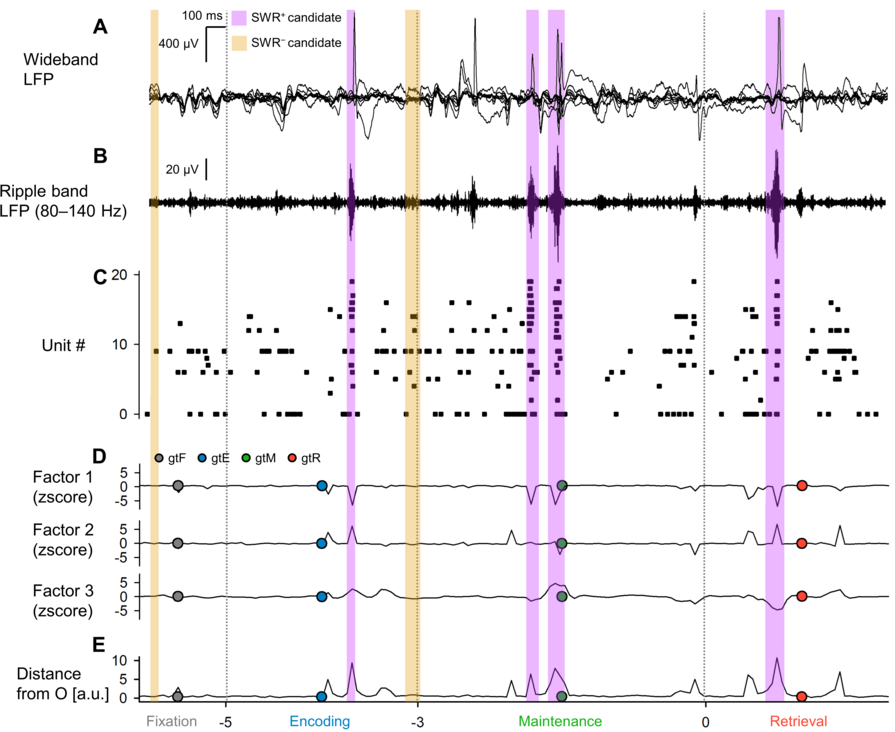
\includegraphics[width=1\textwidth]{./src/figures/.png/Figure_ID_01.png}
        	\caption{\textbf{
Local Field Potentials (LFP), Multiunit Activity, and Neural Trajectories in the Hippocampus During a Modified Sternberg Task
}
\smallskip
\\
\textbf{\textit{A.}} These traces show representative wideband LFP intracranial EEG (iEEG) signals recorded from the left hippocampal head. The subject performed a modified Sternberg working memory task, which includes fixation (1 s, \textit{gray}), encoding (2 s, \textit{blue}), maintenance (3 s, \textit{green}), and retrieval (2 s, \textit{red}). \textbf{\textit{B.}} We then present the corresponding ripple band LFP traces. \textbf{\textit{C.}} The raster plot depicts multiunit spikes taken from the LFP traces, sorted using a spike algorithm \cite{niediek_reliable_2016}. \textbf{\textit{D.}} Subsequently, we illustrate the neural trajectories, which are calculated by GPFA on spike counts per unit with 50-ms bins. Each phase's geometric median is marked by the dot circles. \textbf{\textit{E.}} The trajectory's distance from the origin $O$ is portrayed, with \textit{purple} and \textit{yellow} rectangles indicating the timings for SWR$^+$ candidates and SWR$^-$ candidates (considered as controls for SWR$^+$), respectively.
}
% width=1\textwidth
        	\label{fig:01}
        \end{figure*}
        \clearpage
        \begin{figure*}[ht]
            \pdfbookmark[2]{ID 02}{figure_id_02}
        	\centering
            \includegraphics[width=0.5\textwidth]{./src/figures/.png/Figure_ID_02.png}
        	\caption{\textbf{
State-Dependent Trajectories of Hippocampal Neurons
}
\smallskip
\\
\textbf{\textit{A.}} Neural trajectories within the initial three-dimensional factors derived from the Gaussian Process Factor Analysis (GPFA) are displayed. The smaller dots correspond to coordinates of 50-ms neural trajectory bins, while the larger dots with \textit{black} edges signify the geometric medians for respective stages in the Sternberg working memory task: fixation (\textit{gray}), encoding (\textit{blue}), maintenance (\textit{green}), and retrieval (\textit{red}). \textbf{\textit{B.}} The figure conveys the log-likelihood of the GPFA models versus the count of dimensions used to embed multiunit spikes found in the medial temporal lobe (MTL) territories. In specific, the elbow method pinpointed the optimal dimension to be three. \textbf{\textit{C.}} This panel illustrates the distance of the neural trajectories from the origin ($O$) for the hippocampus (Hipp.), entorhinal cortex (EC), and amygdala (Amy.), against the time elapsed from the probe onset. \textbf{\textit{D.}} The distance of the trajectory from $O$ within MTL regions is displayed. The hippocampus shows the farthest distance, followed by the EC and the Amygdala. \textbf{\textit{E.}} The plot represents inter-phase trajectory distances within the MTL regions.
Abbreviations:
}
% width=0.5\textwidth
        	\label{fig:02}
        \end{figure*}
        \clearpage
        \begin{figure*}[ht]
            \pdfbookmark[2]{ID 03}{figure_id_03}
        	\centering
            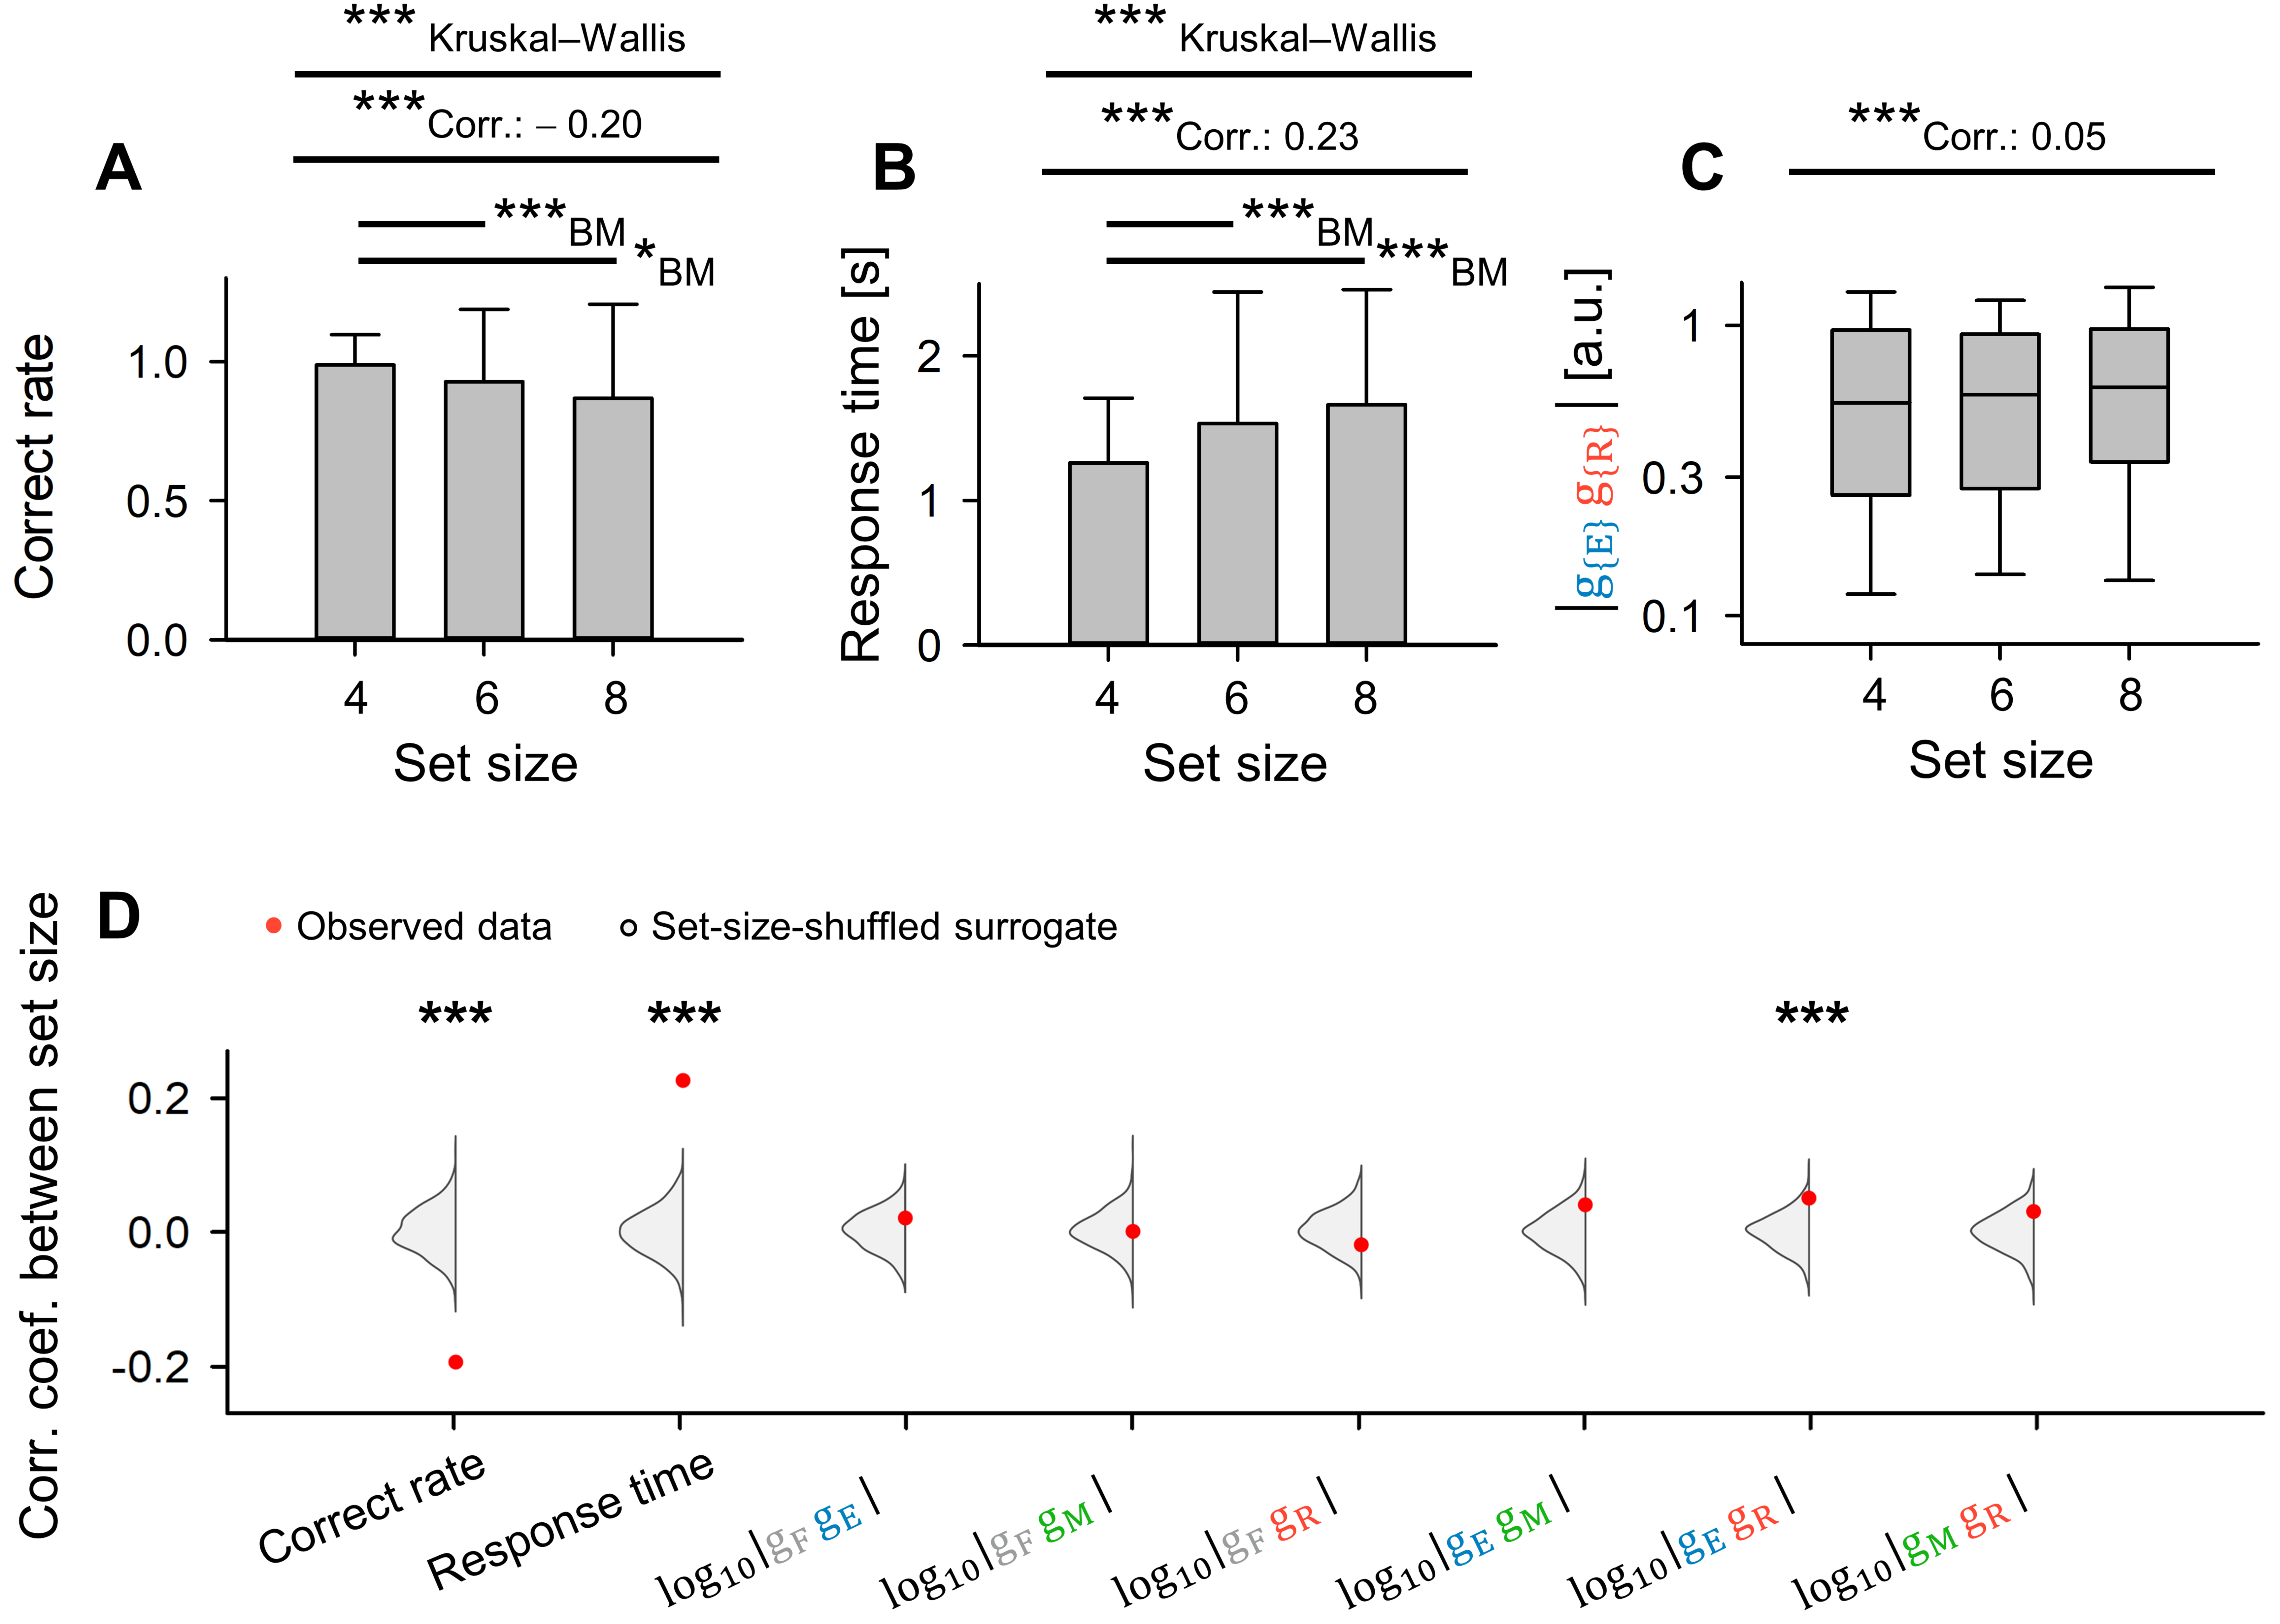
\includegraphics[width=1\textwidth]{./src/figures/.png/Figure_ID_03.png}
        	\caption{\textbf{
Dependency of Trajectory Distance on Memory Load: Encoding and Retrieval States in Hippocampus
}
\smallskip
\\
\textbf{\textit{A.}} The relationship between set size (number of letters that need to be encoded) and correct rate in the working memory task (coefficient = $-0.20$, ***\textit{p} $<$ 0.001). \textbf{\textit{B.}} The correlation between set size and response time (coefficient = 0.23, ***\textit{p} $<$ 0.001). \textbf{\textit{C.}} The impact of set size on the inter-phase distances between the encoding and retrieval phases ($\lVert \mathrm{g_{E}g_{R}} \rVert$) (correlation coefficient = 0.05). \textbf{\textit{D.}} \textit{Red} dots represent experimental observations of correlations between set size and the following parameters: correct rate, response time, $\log_{10}{\lVert \mathrm{g_{F}g_{E}} \rVert}$, $\log_{10}{\lVert \mathrm{g_{F}g_{M}} \rVert}$, $\log_{10}{\lVert \mathrm{g_{F}g_{R}} \rVert}$, $\log_{10}{\lVert \mathrm{g_{E}g_{M}} \rVert}$, $\log_{10}{\lVert \mathrm{g_{E}g_{R}} \rVert}$, and $\log_{10}{\lVert \mathrm{g_{M}g_{R}} \rVert}$. The \textit{gray} kernel density plot illustrates the corresponding set-size-shuffled surrogate (\textit{n} = 1,000) (***\textit{p}s $<$ 0.001).
}
% width=1\textwidth
        	\label{fig:03}
        \end{figure*}
        \clearpage
        \begin{figure*}[ht]
            \pdfbookmark[2]{ID 04}{figure_id_04}
        	\centering
            \includegraphics[width=1\textwidth]{./src/figures/.png/Figure_ID_04.png}
        	\caption{\textbf{
Detection of SWRs in Presumptive CA1 Regions
}
\smallskip
\\
\textbf{\textit{A.}} Two-dimensional UMAP (Uniform Manifold Approximation and Projection) \cite{mcinnes_umap_2018} projection of multiunit spikes during SWR$^+$ candidates (\textit{purple}) and SWR$^-$ candidates (\textit{yellow}). \textbf{\textit{B.}} Cumulative density plot shows silhouette scores, indicative of UMAP clustering quality, for hippocampal regions (see Table~\ref{tab:02} for reference). Note that hippocampal regions with silhouette scores greater than 0.60 (equivalent to the $75^{th}$ percentile) were identified as possible CA1 regions. SWR$^+$ and SWR$^-$ candidates recorded from these speculative CA1 regions were respectively classified as SWR$^+$ and SWR$^-$ (\textit{n}s = 1,170). \textbf{\textit{C.}} The identical distributions of durations are presented for SWR$^+$ (\textit{purple}) and SWR$^-$ (\textit{yellow}), owing to their definitions (93.0 [65.4] ms, median [IQR]). \textbf{\textit{D.}} SWR incidence for both SWR$^+$ (\textit{purple}) and SWR$^-$ (\textit{yellow}) obtained relative to the probe's timing is illustrated as a mean \textpm 95\% confidence interval. However, as the intervals may not be visible due to their narrow range, note that a significant increase in SWR incidence was detected during the initial 400 ms of the retrieval phase (0.421 [Hz], *\textit{p} $<$ 0.05, bootstrap test). \textbf{\textit{E.}} The distributions of ripple band peak amplitudes for SWR$^-$ (\textit{yellow}; 2.37 [0.33] SD of baseline, median [IQR]) and SWR$^+$ (\textit{purple}; 3.05 [0.85] SD of baseline, median [IQR]) are delineated (***\textit{p} $<$ 0.001, the Brunner--Munzel test).
}
% width=1\textwidth
        	\label{fig:04}
        \end{figure*}
        \clearpage
        \begin{figure*}[ht]
            \pdfbookmark[2]{ID 05}{figure_id_05}
        	\centering
            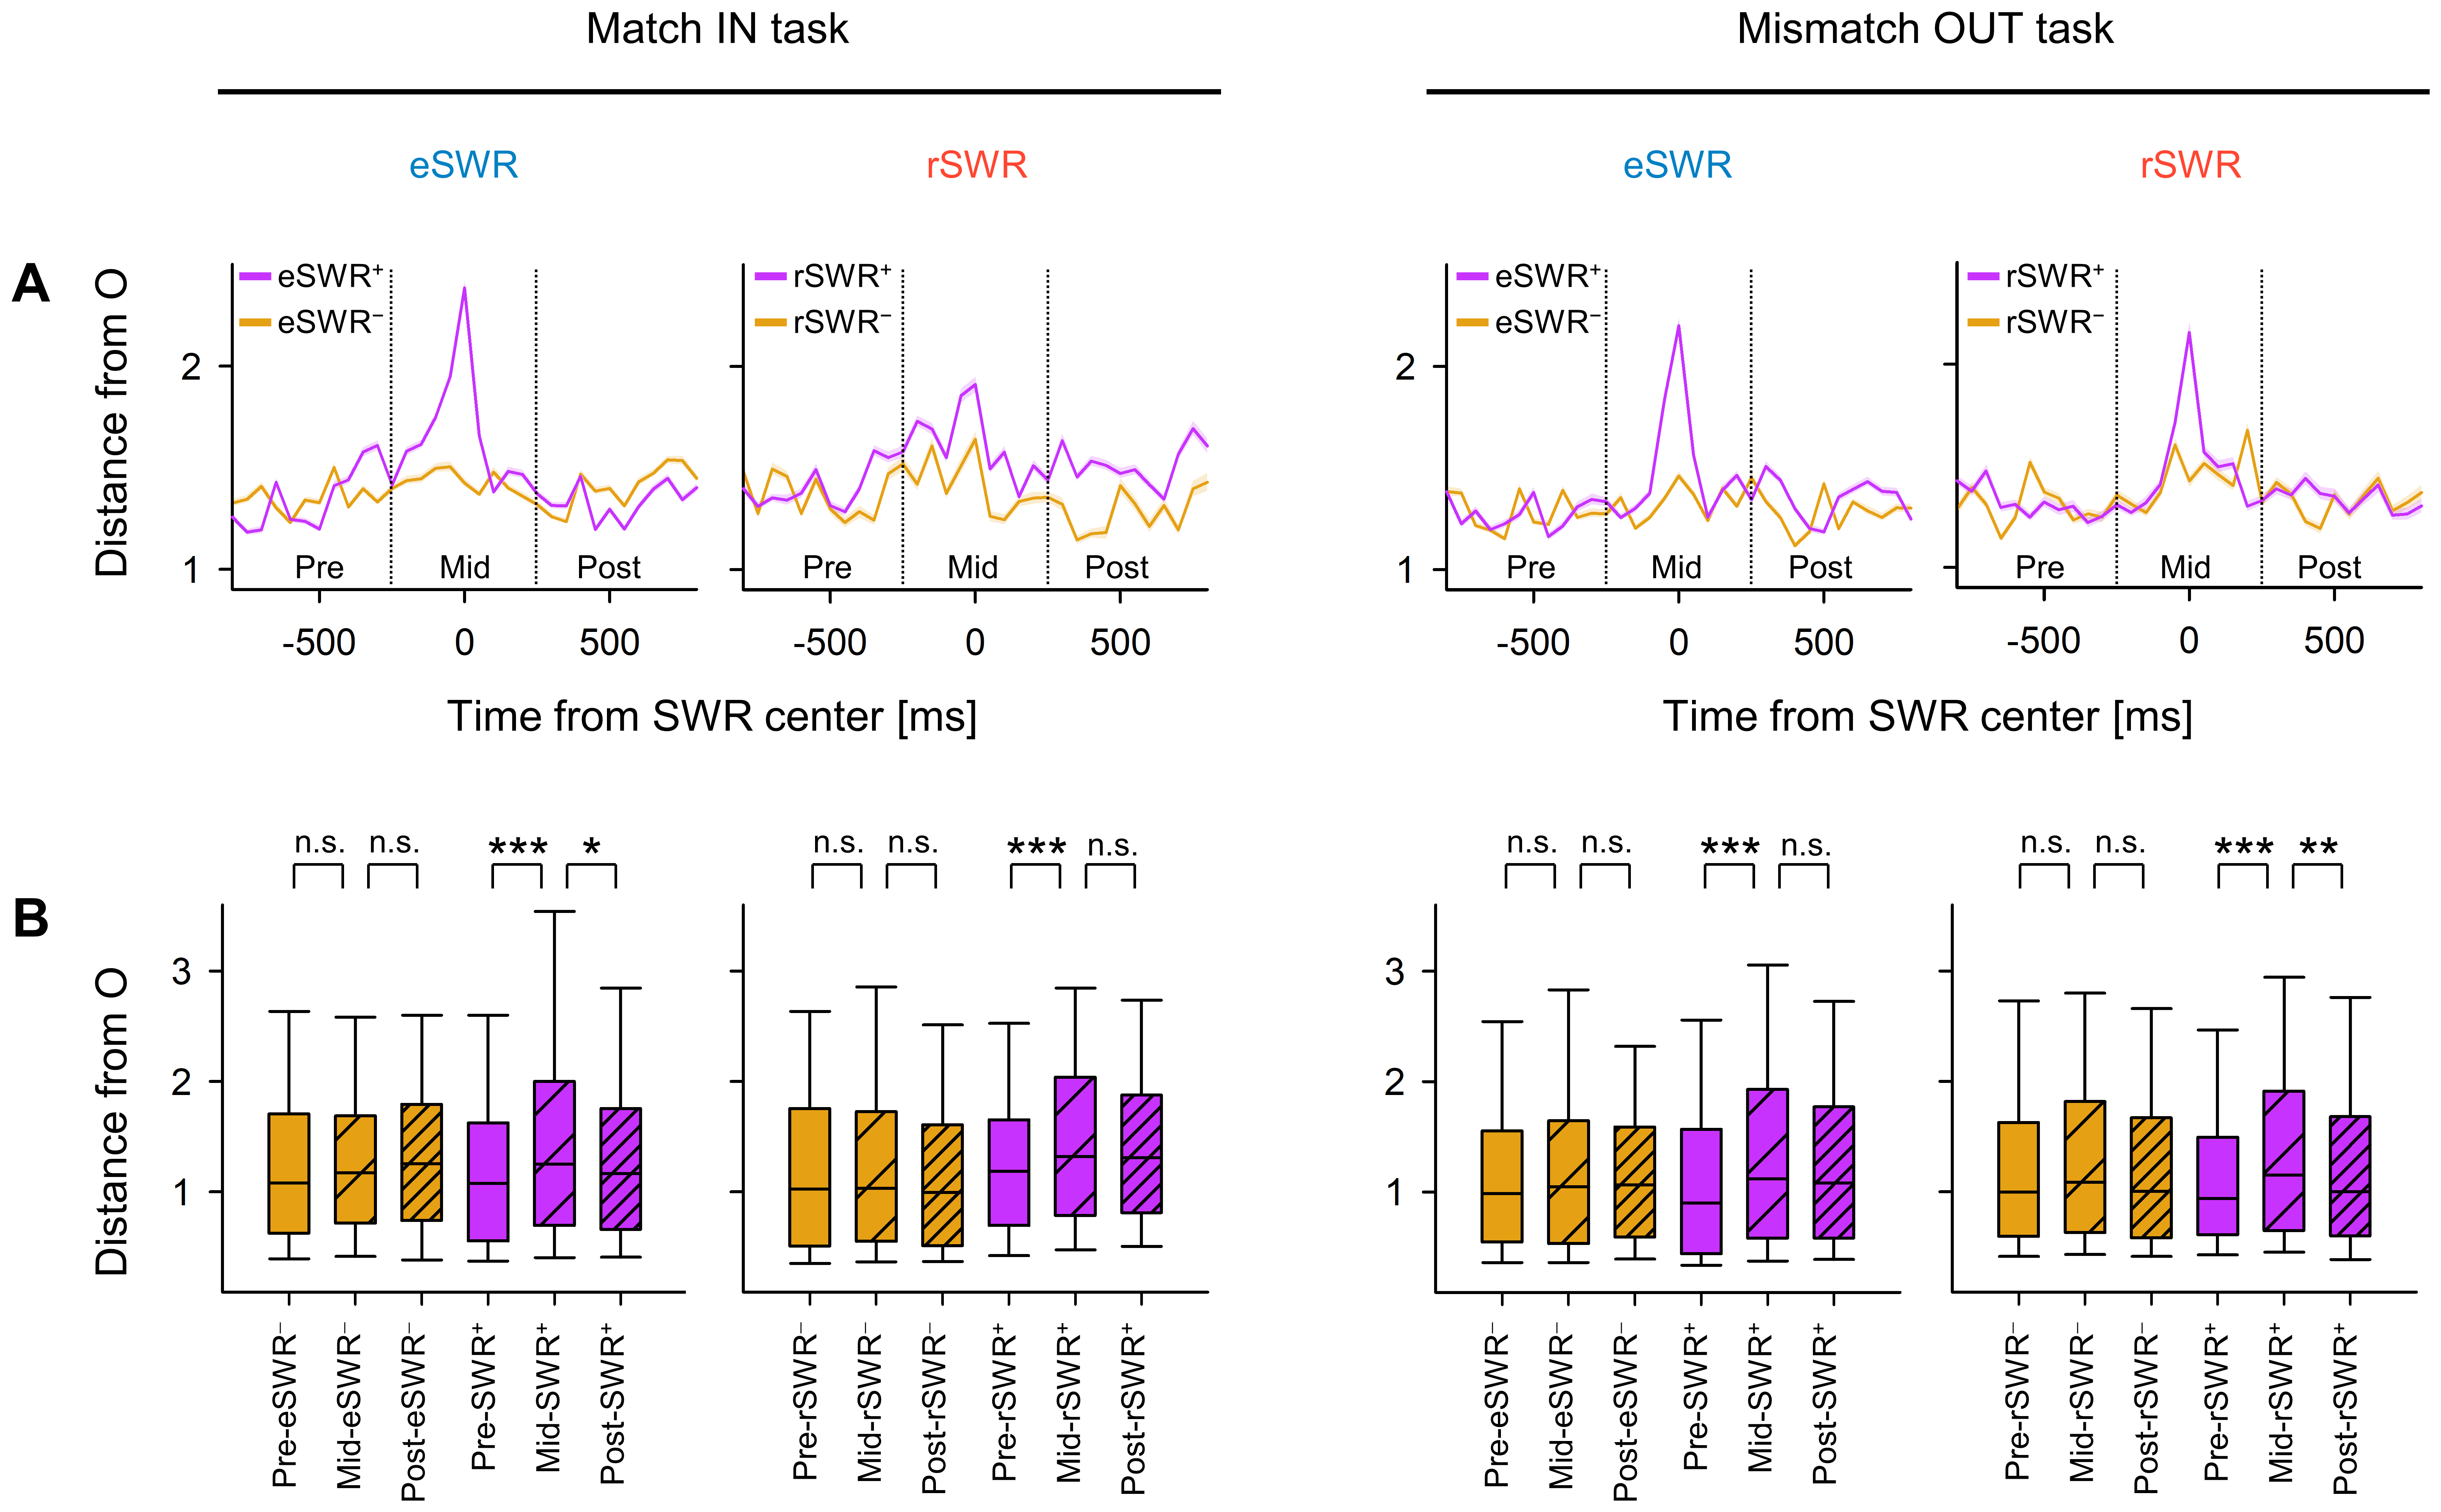
\includegraphics[width=1\textwidth]{./src/figures/.png/Figure_ID_05.png}
        	\caption{\textbf{
Transient Alterations in Neural Trajectory During SWR Events
}
\smallskip
\\
\textbf{\textit{A.}} Displayed is the distance from origin ($O$) of the peri-sharp-wave-ripple trajectory (mean \textpm 95\% confidence interval). The intervals may not be apparent due to their slender ranges. \textbf{\textit{B.}} Shown is the distance from the origin ($O$) during pre-, mid-, and post-SWR periods (*\textit{p} $<$ 0.05, **\textit{p} $<$ 0.01, ***\textit{p} $<$ 0.001; assessed using the Brunner--Munzel test). Abbreviations: SWR, sharp-wave ripple events; eSWR, SWR during the encoding phase; rSWR, SWR while in the retrieval phase; SWR$^+$, positive SWR event; SWR$^-$, control events for SWR$^+$; pre-, mid-, or post-SWR denote the time intervals from $-800$ to $-250$ ms, from $-250$ to $+250$ ms, or from $+250$ to $+800$ ms, all relative to the center of the SWR.
}
% width=1\textwidth
        	\label{fig:05}
        \end{figure*}
        \clearpage
        \begin{figure*}[ht]
            \pdfbookmark[2]{ID 06}{figure_id_06}
        	\centering
            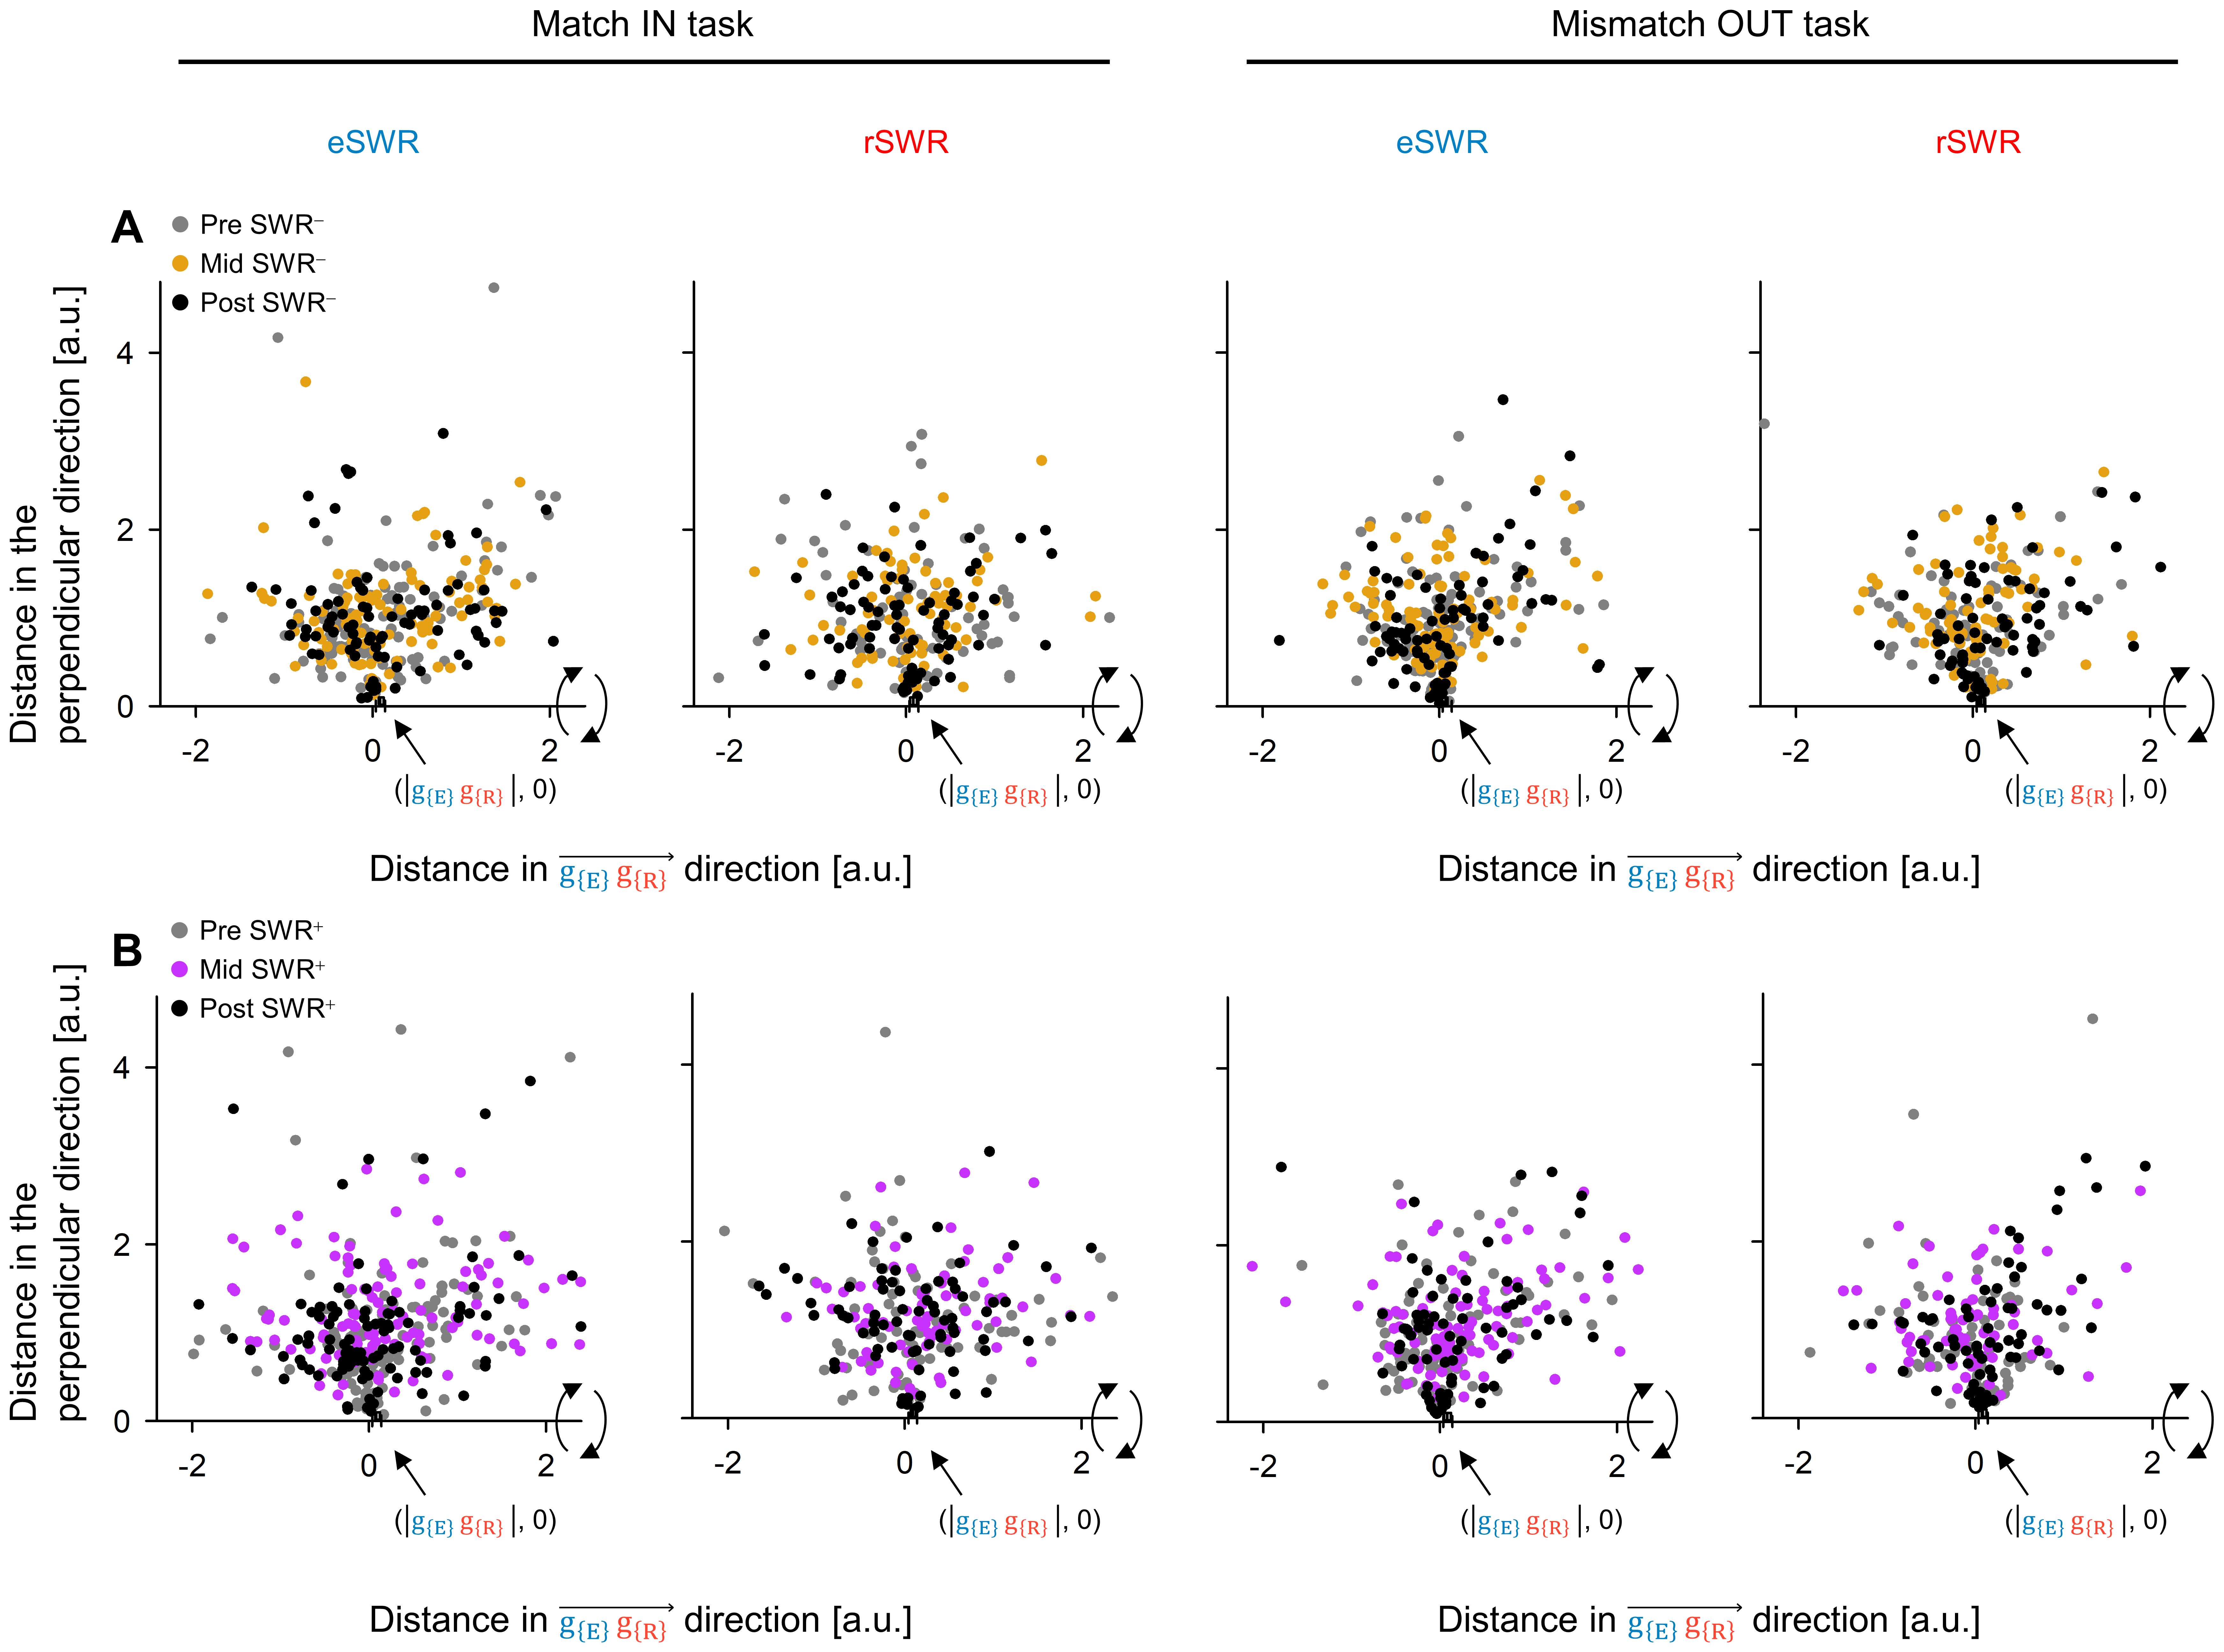
\includegraphics[width=1\textwidth]{./src/figures/.png/Figure_ID_06.png}
        	\caption{\textbf{
Visualization of Neural Trajectories during SWR in Two-Dimensional Spaces}
\smallskip
\\
The panels display hippocampal neural trajectories during SWR as projected onto two-dimensional spaces. \textbf{\textit{A.}} Indicates hippocampal neural trajectories pre-SWR$^-$ (\textit{gray}), mid-SWR$^-$ (\textit{yellow}), and post-SWR$^-$ (\textit{black}). \textbf{\textit{B.}} Represents the equivalents for SWR$^+$ as opposed to SWR$^-$. The $\lVert \mathrm{g_{E}g_{R}} \rVert$ varied among sessions. The projection was applied in the following manner: First, a linear transformation positioned $\mathrm{g_{E}}$ at the origin $O$ (0,0), and $\mathrm{g_{R}}$ at ($\lVert \mathrm{g_{E}g_{R}} \rVert$, 0). The point cloud was then rotated around the $\mathrm{g_{E}g_{R}}$ axis (equivalent to the x axis) for fitting into two-dimensional spaces. Therefore, within these two-dimensional spaces, both the distances from $O$ and the angles preserved the original makeup of the $\mathrm{g_{E}g_{R}}$ axis from the original three-dimensional spaces. Abbreviations: SWR signifies sharp-wave ripple events; eSWR denotes SWR during the encoding phase; rSWR indicates SWR during the retrieval phase; SWR$^+$, marks an SWR event; SWR$^-$ refers to control events for SWR$^+$; pre-SWR, mid-SWR, or post-SWR, reference the time intervals from $-800$ to $-250$ ms, from $-250$ to $+250$ ms, or from $+250$ to $+800$ ms from the center of SWR.
}
% width=1\textwidth
        	\label{fig:06}
        \end{figure*}
        \clearpage
        \begin{figure*}[ht]
            \pdfbookmark[2]{ID 07}{figure_id_07}
        	\centering
            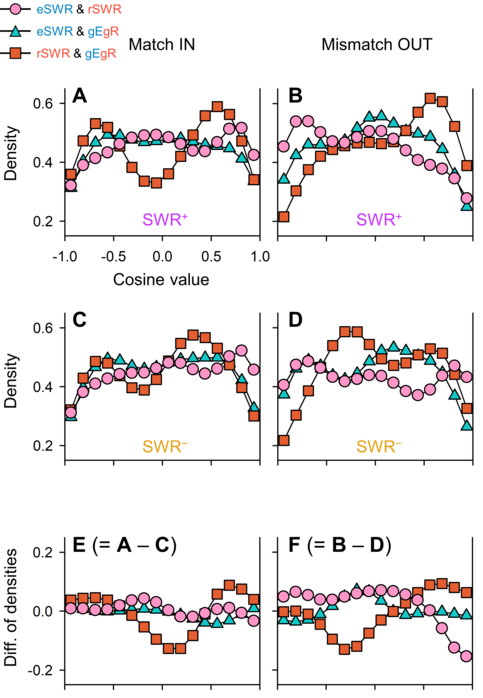
\includegraphics[width=0.5\textwidth]{./src/figures/.png/Figure_ID_07.png}
        	\caption{\textbf{
Directions of Neural Trajectories during SWRs Based on Encoding and Retrieval States
}
\smallskip
\\
\textbf{\textit{A--B}} Kernel density estimation (KDE) distributions of $\protect\overrightarrow{{\mathrm{eSWR^+}}} \cdot \protect\overrightarrow{{\mathrm{rSWR^+}}}$ (\textit{pink circles}), $\protect\overrightarrow{{\mathrm{eSWR^+}}} \cdot \protect\overrightarrow{{\mathrm{g_{E}g_{R}}}}$ (\textit{blue triangles}), and $\protect\overrightarrow{{\mathrm{rSWR^+}}} \cdot \protect\overrightarrow{{\mathrm{g_{E}g_{R}}}}$ (\textit{red rectangles}) in Match In (\textit{A}) and Mismatch OUT tasks (\textit{B}). \textbf{\textit{C--D}} Present the corresponding distributions of $\mathrm{SWR^-}$ instead of those of $\mathrm{SWR^+}$ in \textit{A} and \textit{B}. \textbf{\textit{E--F}} Depict the differences in the distributions of $\mathrm{SWR^+}$ and $\mathrm{SWR^-}$, illuminating the SWR components (\textit{E} = \textit{C} $-$ \textit{A}; \textit{F} = \textit{D} $-$ \textit{B}). Note the biphasic distributions of $\protect\overrightarrow{{\mathrm{rSWR^-}}} \cdot \protect\overrightarrow{{\mathrm{g_{E}g_{R}}}}$, suggesting fluctuations between the encoding and retrieval states during the Sternberg task. Moreover, inverse directionality between $\protect\overrightarrow{{\mathrm{eSWR^+}}}$ and $\protect\overrightarrow{{\mathrm{rSWR^+}}}$ was observed (\textit{pink circles}) in the Mismatch OUT task, but not in the Match IN task \textbf{\textit{E--F}}). Finally, shifts from the retrieval to encoding states were evident in the SWR components in both the Match IN and Mismatch OUT tasks (\textit{red rectangles} in \textit{E} and \textit{F}).
}
% width=0.5\textwidth
        	\label{fig:07}
        \end{figure*}

%%%%%%%%%%%%%%%%%%%%%%%%%%%%%%%%%%%%%%%%%%%%%%%%%%%%%%%%%%%%%%%%%%%%%%%%%%%%%%%%
%% END
%%%%%%%%%%%%%%%%%%%%%%%%%%%%%%%%%%%%%%%%%%%%%%%%%%%%%%%%%%%%%%%%%%%%%%%%%%%%%%%%

\end{document}
